\documentclass[preprint,12pt,authoryear]{elsarticle}

\usepackage{amsmath,amssymb,amsthm}
\usepackage{booktabs}
\usepackage{array}
\usepackage{tabularx}
\usepackage{graphicx}
\graphicspath{{./}{figures/}}
\usepackage{enumitem}
\usepackage[colorlinks=true,urlcolor=blue,linkcolor=blue,citecolor=blue]{hyperref}
\emergencystretch=3em
\setlength{\tolerance}{2000}

\newtheorem{proposition}{Proposition}
\newtheorem{corollary}{Corollary}
\newcommand{\pos}[1]{\left[#1\right]_+}
\newcommand{\dconv}{\Delta b_{\mathrm{conv}}}
\newcommand{\Ups}{\Upsilon_c}
\newcommand{\Eceil}{E_{\mathrm{ceil}}}
\newcommand{\Acmin}{A_c^{\min}}
\newcommand{\tconv}{\tau_{\mathrm{conv}}}

\journal{Ecological Modelling}

\begin{document}

\begin{frontmatter}

\title{A rising biocapacity total can mask ecological-capital land drawdown: a two-land model}

\author[1]{Amin Abaee\corref{cor1}}
\cortext[cor1]{Corresponding author. Email: \href{mailto:amin_abaee@ut.ac.ir}{amin\_abaee@ut.ac.ir}. ORCID: \href{https://orcid.org/0000-0002-0019-1842}{0000-0002-0019-1842}.}
\affiliation[1]{organization={Independent Researcher}, city={Tehran}, country={Iran}}

\begin{abstract}
Biocapacity is reported as an aggregate, despite wide differences in yield and regeneration among its constituent land classes. A rising total alone cannot reveal whether its composition has shifted. We examine this accounting problem with a two-land model that includes delayed ecological regeneration, population response, and an explicit projection of the quality state onto an imposed admissible interval. The quality ceiling is a model-imposed admissibility bound, not an estimated ecological threshold. Under the model's baseline conditions, a shortfall-triggered transfer to fast-provisioning land with a higher annual contribution per hectare adds to model biocapacity through the conversion term even as capital-land area falls. In a representative run, total model biocapacity rises $39\%$ as capital-land area falls $46.16\%$; the modeled capital-land contribution falls $51.72\%$. On the reduced fixed-demand comparison, the equality relation reaches the minimum-area floor without a fold or critical slowing; this result does not characterize the separate surplus no-conversion family or every trajectory of the delayed model. Separately, NFA Edition 2026 account values for 1961--2023 show total world biocapacity up $24.86\%$, while $B/P$ falls $52.71\%$ and the production footprint per person rises $16.73\%$. Cropland contributes $+24.06$ percentage points, Forest biocapacity $-5.95$, and built-up land $+7.44$ as an accounting class. These account movements are not measurements of physical stocks. Component values help interpret the aggregate.

\end{abstract}

\begin{keyword}
\footnotesize
biocapacity \sep ecological footprint \sep land-use conversion \sep aggregation \sep identifiability \sep critical slowing down \sep delay differential equations \sep carrying capacity
\end{keyword}

\end{frontmatter}

\section{Introduction}\label{sec:intro}

In ecology, \emph{carrying capacity} describes the population a resource base can sustain. Many models treat it as a fixed ceiling, in part because it is difficult to estimate \citep{Cohen1995}. If resource use changes the basis of future production, however, a fixed ceiling may not capture that change. This raises a measurement question: can a headline environmental metric report a rising total while a productive land class loses area?

The National Footprint and Biocapacity Accounts (NFA) report biological supply as biocapacity and human demand as the Ecological Footprint. Both are expressed in global hectares (gha), which adjust area for biological productivity relative to the world average in a given year; the annual basis is implicit \citep{GFNStandards2009,GFNGuidebook2019}. Because a global hectare combines area and productivity, a change in the total does not by itself show whether yields, area, or the mix of land uses changed. Has productivity increased, has the area in production shifted, or has the composition of the account changed?

In composite-indicator theory, this ambiguity is called \emph{compensation}: a gain in one component can offset a loss in another \citep{Nardo2008,Becker2017,Fischer2022}. The aggregate remains useful, but reading it alone can conceal component changes. Related critiques discuss the interpretation of the Ecological Footprint and biocapacity accounts \citep{Blomqvist2013,GiampietroSaltelli2014,vdBerghGrazi2015,Galli2016}.

Most human--environment models summarize nature as an aggregate stock or a unified feedback. Examples include the \emph{World3} simulations \citep{Meadows1972,Meadows1974,Meadows2004}, models of Easter Island \citep{BranderTaylor1998,Anderies2000}, and coupled Earth-system frameworks \citep{Motesharrei2016,Donges2017,CalvinBondLamberty2018,HendersonLoreau2018}. Other work debates whether human carrying capacity is fixed, variable, or useful as a concept \citep{Cohen1995,vdBerghRietveld2004,Simon1996,Meyer1994,MeyerAusubel1999,Dasgupta2021}; global demographic assessments often project population separately from environmental constraints \citep{UN2022}. Land-use studies, meanwhile, document conversion among forests, grasslands, wetlands, and cropland \citep{Haberl2007,Krausmann2013,Erb2017}. Together, these literatures motivate a narrower question: what can one biocapacity total reveal when land classes differ in yield and regeneration?

\paragraph{Analogies} To make the accounting issue concrete, imagine an orchard with fast-provisioning ground, such as intensively managed beds, beside slower-renewing ground with trees and living soil. Annual harvest is a \emph{flow}; trees, roots, and soil are assets that support future flows. In our model, a shortfall can trigger a transfer from ecological-capital land to fast-provisioning land. If the receiving class has a higher annual contribution per hectare in that scenario, the conversion term adds to $B$ at the margin while capital-land area $A_c$ falls; other flows can offset that increment. This is a conditional model mechanism, not evidence that NFA accounts measure physical stocks or that a particular real-world conversion occurred. Replanting may restore a later harvest, but it is not a one-for-one measure of the condition or recovery of the distinct assets represented by the model's capital-land class. The analogy separates current output from the state of its productive base; it does not assert that the classes map directly to NFA categories.

A second analogy separates observed service from structural condition: an elevator rated for ten people might continue operating while carrying fourteen, but the ride itself does not establish whether repeated overloading has changed the cable's safety margin. Continued service is not a measurement of structural condition, nor does the analogy predict inevitable failure. Related material-ledger work discusses a broader flow--stock masking problem; here we study its composition-specific form in a biocapacity model \citep{Abaee2026c}.

\paragraph{Research questions} This paper addresses three questions:
\begin{enumerate}
  \item \textbf{The masking dynamic:} Under what conditions can conversion raise total model biocapacity while $A_c$ declines, how long can this divergence last, and can the aggregate identify the land shift?
  \item \textbf{System trajectory:} Under the model's stated assumptions, does drawdown involve a fold, hysteresis, or critical slowing, or does the reduced comparison follow another path?
  \item \textbf{Limits and recovery:} What limits drawdown under fixed demand, and what modelled process allows capital-land area to recover?
\end{enumerate}

\paragraph{Core contributions} We make three contributions:
\begin{itemize}
  \item We construct a dynamic two-land model that conserves total area, represents capital-land quality separately from area, and includes delays in ecological regeneration and demographic response.
  \item We derive the condition under which a conversion term raises aggregate biocapacity while $A_c$ falls. In a reduced fixed-demand comparison, the balance relation reaches the area floor without a fold or critical slowing; realized paths in the delayed model remain history-dependent. These are conditional model results, not general claims about observed ecosystems.
  \item We decompose NFA Edition 2026 account values for 1961--2023 and examine a separate cropland-area/yield proxy. The account series show a compositional change, not a census of physical ecological stocks.
\end{itemize}

Finally, we derive five testable empirical predictions. The model parameters are representative rather than fitted, so simulations illustrate conditional mechanisms rather than historical forecasts. Aggregate biocapacity is therefore most informative when read alongside its component accounts.

\section{Methods}\label{sec:model}

\subsection{A two-land model with conserved area and ecosystem quality}\label{sec:equations}

To examine how an aggregate indicator can mask a change in composition, we divide total bioproductive area $A_{tot}$ among three mutually exclusive classes:
\begin{itemize}
  \item \textbf{Fast-provisioning land} ($A_f$): cropland and other intensively managed systems, represented by their annual contribution.
  \item \textbf{Ecological-capital land} ($A_c$): forest, soil, wetland, and long-rotation systems grouped into one effective class, rather than treated as a single real land type.
  \item \textbf{Reserve land} ($A_r$): fallow, retired, or not-yet-allocated area.
\end{itemize}
The three areas sum to $A_{tot}$. The model also assigns capital land a separate, uncalibrated, model-defined quality index $q\in[0,q_{\max}]$. This effective state changes the modeled annual contribution per hectare; it is not a direct measurement of biomass density, soil integrity, or ecological health. The baseline bound $q_{\max}=1$ is imposed for admissibility, not estimated as an ecological threshold. The raw regeneration-rate function is logistic:
\begin{equation}\label{eq:Gc}
G_c(q)=\rho_c\,q\left(1-\frac{q}{q_{\max}}\right),
\end{equation}
Capital land's annual contribution per hectare combines a direct-yield term with a term linked to quality growth:
\begin{equation}\label{eq:Ups}
\Ups(q)=b_c+b_{G,c}\,G_c(q),
\end{equation}
where $b_c$ is direct yield and $b_{G,c}$ converts the quality-growth term into annual account value. The fast- and capital-land contributions, $Y_f$ and $Y_c$, sum to total model biocapacity:
\begin{equation}\label{eq:B}
B=Y_f+Y_c=b_f A_f+\Ups(q)\,A_c ,
\end{equation}
Here $b_f$ is fast-land contribution per hectare. Model $B$ is an annual account-equivalent amount in gha, with the annual basis implicit \citep{GFNStandards2009,GFNGuidebook2019}.

\paragraph{Demand, shortfalls, and land conversion} Total demand is $E=eP$, where $P$ is population and $e$ is the constant footprint per person (gha per person; $\mathrm{cap}$ denotes one person in the equations and tables). The shortfall $S$ is the demand not met by the human-available shares of the two land contributions:
\begin{equation}\label{eq:S}
S=\pos{E-\sigma_f Y_f-\sigma_c Y_c},
\end{equation}
The positive-part operator is $\pos{x}=\max(x,0)$; baseline availability fractions are $\sigma_f=\sigma_c=1$. When $S>0$, the model transfers capital land to fast-provisioning land at a finite rate:
\begin{equation}\label{eq:uc}u_c=\frac{1}{\tconv}\min\!\left(\frac{S}{b_f},\;A_c-\Acmin\right)\qquad[\mathrm{ha\,yr^{-1}}],
\end{equation}
The ratio $S/b_f$ is the fast-land area required to cover the shortfall under this model rule; $\Acmin$ is the lower area bound, and $\tconv$ sets the conversion timescale. This transfer is a specified response rule, not a reconstruction of observed land-clearing decisions.

\paragraph{Land flows and asymmetric restoration} Land moves among classes through one-to-one area transfers:
\begin{align}
\dot A_c&=-u_c+R_{rc},\label{eq:Ac}\\
\dot A_f&=u_c+\mu A_r-\eta_f A_f,\label{eq:Af}\\
\dot A_r&=-\mu A_r+\eta_f A_f-R_{rc},\label{eq:Ar}
\end{align}
The flow $\mu A_r$ moves reserve area into fast use, while $\eta_f A_f$ retires fast land to reserve. Reserve land returns to the capital-land class only through the surplus-gated restoration flow $R_{rc}$:
\begin{equation}\label{eq:Rrc}
R_{rc}=\chi_r\,A_r\,\pos{B-E}.
\end{equation}
Restoration is therefore asymmetric in the model: fast land may be retired into reserve, but reserve returns to ecological-capital use only when the modeled surplus is positive and the restoration flow is active. A closed shortfall alone does not restore capital-land area.

\paragraph{Delays, model debt, and demographics} Quality responds to its delayed value through projection of the regeneration vector field onto the tangent cone of $K_q=[0,q_{\max}]$. Population responds to carrying capacity evaluated at $t-\tau_p$; the delay is in the capacity input, not in population itself in its crowding term. The model also tracks a leaky deficit state $D$ that affects fast-land yield:
\begin{align}
\dot q&=\Pi_{T_{K_q}(q(t))}G_c\big(q(t-\tau_g)\big),\label{eq:q}\\
\dot P&=rP\left(1-\frac{P}{K(t-\tau_p)}\right),\qquad K=\max(B/e,\,K_{\min}),\label{eq:P}\\
b_f&=\big(b_{f0}+T_b(t)\big)\,e^{-\alpha D},\label{eq:bf}\\
\dot D&=\pos{E-B}-\eta D,\label{eq:D}\\
T_b(t)&=\omega_{Tb}\,\frac{\Delta b}{1+e^{-\kappa_w(t-t_{wave})}},\qquad \omega_{Tb}\in\{0,1\}.\label{eq:Tb}
\end{align}
Here $K_q=[0,q_{\max}]$, $T_{K_q}(q)$ is its tangent cone at the current state, and $\Pi$ is Euclidean projection onto that cone. We interpret the quality equation as an absolutely continuous solution, almost everywhere, with $\rho_c>0$ and an admissible continuous history $q(s)=\phi(s)\in K_q$ for $s\in[-\tau_g,0]$. Since $G_c(x)\ge0$ for $x\in K_q$, the projected law agrees with the raw delayed rate below the upper bound and sets outward growth to zero at $q=q_{\max}$; at $q=0$ the vector field is nonnegative. The cap is a mathematical admissibility constraint, not an empirically identified biological saturation mechanism.
Areas $A_f$, $A_c$, and $A_r$ are measured in hectares; $B$, $E$, and $S$ are annual account amounts in gha, with the annual basis implicit. $D$ is measured in gha\,yr; both $\dot D$ and $\eta D$ are in gha. It is an internal model state driven by aggregate deficit, not an area, a physical stock, or an NFA-reported quantity. The optional technology boost $T_b$ raises fast-land yield along a bounded logistic curve. It is off in the baseline, figures, and tables, and appears only in the matched comparison in SI~\S S8. The dynamic states are $A_f$, $A_c$, $q$, $P$, and $D$; timber liquidation and direct restoration from fast land to capital land are not active in the reported runs (SI~\S S1).

\paragraph{Core system feedbacks} The equations permit two conditional feedbacks:
\begin{enumerate}
  \item \textbf{Compositional-yield feedback.} When fast land contributes more per hectare than capital land ($b_f>\Ups(q)$), conversion raises $B$ at the margin while reducing $A_c$. With endogenous population, higher $B$ can raise delayed carrying capacity $K$ and later population and demand, potentially creating another shortfall. Maintenance, retirement, quality change, and the other model terms also affect $B$; this is a model feedback, not an empirical causal finding.
  \item \textbf{Deficit--yield feedback.} A shortfall adds to $D$, while repayment draws it down. As $D$ grows, modeled fast-land yield $b_f$ falls; this can reduce $B$ and deepen the shortfall. The state $D$ is the model's leaky deficit measure, not a direct measure of nutrient depletion, aquifer overdraft, or other physical processes.
\end{enumerate}

\subsection{Parameter selection and empirical grounding}\label{sec:params}

Table~\ref{tab:params} summarizes the baseline parameter values and their evidence status. Parameters are representative rather than econometrically fitted; the model is designed to isolate structural mechanisms, not to generate precise historical forecasts. To keep the model tractable, it consolidates forests, soils, wetlands, and other slow-renewing systems into one effective capital-land class, although their extent, condition, yields, and recovery dynamics differ substantially. Published forest, fish-stock, and soil studies use heterogeneous recovery definitions and document system-specific responses (SI~\S S5.5) \citep{Poorter2016,HutchingsReynolds2004,Neubauer2013,Poeplau2011}. We do not refit a common recovery curve or compute harmonized $t_{50}$ or $\tau_r$ values from those records here. They are measurement and future-modeling precedents only; they do not estimate $\rho_c$ or $\tau_g$, validate the present generic quality equation, or identify its parameters.

Two data-based quantities provide context for cropland but do not calibrate the model: the NFA cropland account value per unit area and a separate cereal-yield/cropland-area proxy (SI~\S S5). Their boundaries do not map one-to-one onto model fast land, and neither is a fitted value of $b_f$ or a direct measure of ecological capital. Finally, the baseline assumes $b_f-\Ups(q)>0$. This is an explicit conditional modeling regime for examining when a short-term contribution premium can mask a change in land composition, not a universal empirical claim.

\begin{table}[!htbp]
\centering\footnotesize
\renewcommand{\arraystretch}{0.80}
\caption{Baseline parameter values and evidence status. Representative values are effective, lumped quantities; the NFA account/area quotient is descriptive, not a physical-yield measurement. Extension parameters are active only in scenarios specified in this table or the SI. Symbols and units are listed in SI~\S S1.}
\label{tab:params}
\setlength{\tabcolsep}{4pt}
\begin{tabularx}{\textwidth}{@{}>{\raggedright\arraybackslash}p{0.13\textwidth} >{\raggedright\arraybackslash}p{0.2\textwidth} >{\raggedright\arraybackslash}X >{\raggedright\arraybackslash}p{0.26\textwidth}@{}}
\toprule
Parameter & Value & Meaning & Status \\
\midrule
$\rho_c$ & $0.08$\,yr$^{-1}$ & quality-regeneration scenario rate & scenario setting; not estimated \\
$b_{f0}$ & $0.85$\,gha\,ha$^{-1}$ & base fast-land yield per hectare & representative (2026 NFA account value/area quotient $\approx1.045$ in 1961; not a physical-yield measure) \\
$b_c$ & $0.05$\,gha\,ha$^{-1}$ & capital-land direct yield & representative \\
$b_{G,c}$ & $0.8$\,gha\,yr\,ha$^{-1}$ & regeneration-value coefficient for capital land & representative \\
$q_{\max}$ & $1.0$ (dimensionless) & imposed quality admissibility bound & not an estimated ecological threshold \\
$\mu$ & $0.06$\,yr$^{-1}$ & cropland maintenance (reserve$\to$fast) & representative \\
$\eta_f$ & $0.05$\,yr$^{-1}$ & fast-land retirement (fast$\to$reserve) & representative \\
$\tconv$ & $1.0$\,yr & conversion time constant & representative \\
$\alpha$ & $0.03$\,gha$^{-1}$\,yr$^{-1}$ & degradation of $b_f$ per unit debt & representative \\
$\eta$ & $0.05$\,yr$^{-1}$ & debt-repayment rate ($>0$) & representative \\
$e$ & $0.55$\,gha\,cap$^{-1}$ & per-capita footprint (constant) & representative \\
$r$ & $0.02$\,yr$^{-1}$ & intrinsic population growth & representative \\
$\tau_g,\ \tau_p$ & $20,\ 25$\,yr & regeneration and demographic delay scenarios & scenario settings; $\tau_p$ lumps institutional lags \\
$A_{tot}$ & $2.5$\,ha & total bioproductive area & normalization \\
$\sigma_f,\ \sigma_c$ & $1,\ 1$ (dimensionless) & human-available shares of annual account amounts & baseline ($<1$: reservation extension) \\
$\chi_r$ & $0.10$\,gha$^{-1}$\,yr$^{-1}$ & surplus-gated restoration coefficient & on with endogenous demand; off under frozen demand \\
$\Acmin$ & $0.05$\,ha & capital-land area floor & enforced by conversion-rate law \\
$A_r^{\min}$ & $0.10$\,ha & reserve monitoring threshold & not enforced by the update \\
$K_{\min}$ & $0.02$\,cap & carrying-capacity floor & imposed in definition of $K$ \\
$\Delta b$, $\kappa_w$,\newline $t_{wave}$ & $1.0$\,gha\,ha$^{-1}$, $0.1$\,yr$^{-1}$,\newline $40$\,yr & technology wave & off in baseline; active only in the matched SI S8 experiment \\
\bottomrule
\end{tabularx}
\end{table}

\subsection{Data and empirical measures}\label{sec:data}

Our empirical analysis uses the National Ecological Footprint and Biocapacity Accounts (NFA), Edition 2026, results and metadata version 1.0 \citep{Lo2026NFA}. We analyse complete world observations for 1961--2023 and exclude preliminary estimates for 2024--2025. A 1961--2022 sensitivity check uses the same account edition and population series, so the data vintage is held constant across the two windows.

From the workbook's \texttt{world\_data} sheet, we extract total biocapacity $B$ (\texttt{biocap\_total\_gha}), the Global Ecological Footprint of Production $E_{\mathrm{prod}}$ (\texttt{efp\_total\_gha}), and UN PopStat population $P$ (\texttt{pop\_1000\_persons}). Population is converted from thousands to persons. Per-person measures are calculated from unrounded totals rather than the workbook's rounded per-person columns; ratios, indices, and log changes are dimensionless.

\paragraph{Accounting categories and physical stocks} We retain the five workbook labels: \emph{Cropland}, \emph{Grazing land}, \emph{Forest biocapacity}, \emph{Fishing grounds}, and \emph{Built-up land}. These are account values, not measurements of biomass, soil condition, wetland extent, fish biomass, or model area $A_c$. Built-up land is an NFA accounting class, not ecological capital. We therefore interpret movements among categories as changes in account composition, not as direct observations of physical ecosystems or of the model's capital-land stock.

\paragraph{Auxiliary cropland proxy} As a separate comparison, we pair Our World in Data's FAOSTAT-derived world cropland-area series (arable land plus permanent crops) with cereal yield \citep{OWIDCropland2026,OWIDCereal2026}. Cereal yield is a limited productivity indicator, not a measure of all-crop output or an NFA yield factor. We scale the proxy to the NFA cropland share of total biocapacity in 1961, calculate the crop-account proxy $X_t=\hat b_{f,t}A_{f,t}$, and define the remainder as $C_t=B_t-X_t$. Here $A_{f,t}$ denotes observed cropland area for this auxiliary calculation, not the model state. The scaling makes this an assumed account split, not an independent measurement of the model's fast-land contribution or of physical capital. The remainder absorbs differences in boundaries, categories, and calibration; it is not $\Ups(q)A_c$. SI~\S S5 reports the proxy and its calibration sensitivity. We infer no physical-stock trend from it.

\paragraph{Total and per-person change} We use the exact identity
\begin{equation*}
\Delta\ln B=\Delta\ln(B/P)+\Delta\ln P
\end{equation*}
to separate the scale change in total biocapacity from the change in biocapacity per person. This is an accounting identity, not a causal model of biocapacity production.

\subsection{Numerical implementation}\label{sec:numerics}

We integrate the delay equations by the method of steps with an explicit first-order Euler scheme. At step $k$, current states are read at $t_{k-1}$; time-dependent inputs and delayed values are evaluated at $t_k$, with linear interpolation of the delayed $q$ and $B$ histories. The raw delayed quality velocity is projected onto $T_{K_q}(q(t_{k-1}))$ before the Euler update; the updated quality is then clipped to $K_q$ as a finite-step safeguard. The explicitly enforced state bounds are applied, reserve area is reconstructed as $A_r=A_{tot}-A_f-A_c$, and the updated $B$ is stored in the delay history. The reserve threshold $A_r^{\min}$ is monitored rather than projected; the optional $A_f^{\max}$ ceiling is not active in reported runs. The positive-part operator is evaluated exactly. Baseline demonstration and high-resolution threshold runs use $\Delta t=0.05$\,yr; broader drawdown sweeps use $0.1$\,yr, with selected thresholds rechecked at $0.05$\,yr.

Pre-run histories are initialized over the full longest active delay window, $[-\max\{\tau_g,\tau_p\},0]$, as $q(s)=q_0$ and $B(s)=B_0$, with $B_0$ calculated from the initial state. In the matched technology-wave experiment (SI~\S S8), both runs share the no-wave prehistory; the active $T_b(0)$ changes current $B(0)$ and subsequent wave-adjusted $B(t)$ enters the delayed carrying-capacity input $K(t-\tau_p)$. The enforced state bounds are $A_c\ge\Acmin$, $A_f\ge0$, $q\in K_q$, $P,D\ge0$, and $K\ge K_{\min}$. The reserve threshold $A_r^{\min}=0.10$\,ha is a post-hoc monitoring criterion, not an invariant enforced by the update; $A_f^{\max}$ is not imposed in the reported runs.

A finite-step consistency test compared post-Euler quality clipping with explicit tangent-cone projection before the Euler update. At $\Delta t=0.05$\,yr and $T=100$\,yr, using the Figure~\ref{fig:model} initial state and parameters, the tested arrays for $A_f$, $A_c$, $q$, $P$, $D$, $A_r$, $B$, $E$, and $T_b$ were exactly equal at $\tau_g=5,20,40$\,yr. For the continuous baseline quality path at $\tau_g=20$ or $40$\,yr, $q(t)=\min(1,0.9+0.0072t)$; its maximum piecewise-linear error fell from $7.1\times10^{-5}$ at $\Delta t=0.1$\,yr to $8.8\times10^{-6}$ at $0.0125$\,yr. In the full frozen-demand Figure~\ref{fig:model} case, halving $\Delta t$ from $0.05$ to $0.025$\,yr reduced maximum absolute differences against a $0.003125$\,yr reference from $0.00221$ to $0.00102$\,ha for $A_c$, $0.00180$ to $0.000831$\,gha for $B$, $0.000252$ to $0.000118$\,cap for $P$, and $0.00200$ to $0.000924$\,gha\,yr for $D$ (SI~\S S3). These checks establish equality only for the enumerated cases and show smaller differences under timestep refinement; they are not a universal error bound or proof of convergence for all settings.

All reported baseline trajectories use the projected delayed-quality law in Eq.~\eqref{eq:q}. SI~\S S3 presents the current-quality comparator $G_c(q(t))$ only as a sensitivity check; it is not the selected model.
\section{Results}\label{sec:results}

\subsection{When conversion raises the total as capital land declines}\label{sec:mask}

For a given capital-land quality level $q$, its annual contribution per hectare, $\Ups(q)$, is a concave quadratic. It peaks at $q^*=q_{\max}/2$; with the baseline parameters, the maximum is $0.066$\,gha\,ha$^{-1}$. The quality-related term contributes $0.016$ of that value, while direct yield contributes $0.05$\,gha\,ha$^{-1}$; the direct-yield component is larger in this case.

Conversion changes the aggregate according to the gap between the annual account contribution of one fast-land hectare and the effective value of one capital-land hectare. We call this gap the \emph{composition diagnostic}:
\begin{equation}\label{eq:dconv}
\dconv(q,D)=b_f(D)-\Ups(q).
\end{equation}
At baseline, $\dconv$ equals $+0.787$, $+0.784$, and $+0.794$\,gha\,ha$^{-1}$ at $q=0.3$, $0.6$, and $0.9$. Each lies in the composition-premium regime ($\dconv>0$), where conversion adds to the aggregate at the margin. At $\dconv=0$ the contribution is first-order neutral; below zero, it is a composition-discount. These labels describe the conversion term only. Maintenance, retirement, quality change, and other flows still determine the net change in $B$. At any given quality level, that contribution changes linearly with $A_c$; it has no interior maximum with respect to area.

\begin{proposition}[Conversion, aggregate change, and what the total can reveal]\label{prop:mask}
Let $T_b\equiv0$, $R_{rc}\equiv0$ and hold $D$ fixed, so that $b_f$ is constant. Along any solution of \eqref{eq:B}--\eqref{eq:q},
\begin{equation}\label{eq:identity}
\dot B=\dconv(q)\,u_c+b_f\big(\mu A_r-\eta_f A_f\big)+b_{G,c}\,G_c'(q)\,A_c\,\dot q .
\end{equation}
\begin{enumerate}[label=(\roman*)]
\item During conversion ($u_c>0$), $A_c$ falls when restoration is off. The conversion component of $\dot B$ is $\dconv(q)u_c$, positive exactly when $\dconv(q)>0$. When maintenance balances retirement ($\mu A_r=\eta_fA_f$) and quality is unchanged ($\dot q=0$), it is the only term in \eqref{eq:identity} and determines the sign of net $\dot B$. These restrictions are sufficient, not necessary; otherwise the net sign depends on the magnitudes of all active terms, including the conversion contribution.
\item At any instant in the reduced comparison—with fixed demand and debt, baseline availability shares, balanced maintenance and retirement, and no quality change—a positive $\dconv$ makes the shortfall shrink while conversion is active. This is a pointwise statement: with $R_{rc}=0$, $M=\mu A_r-\eta_fA_f$ evolves as $\dot M=-(\mu+\eta_f)M-\eta_fu_c$, so $M=0$ is not invariant when $u_c>0$. The pointwise identity therefore does not imply that the shortfall closes or that the trajectory reaches the area floor under the displayed land flows.
\item At fixed $b_f>0$ and $q$, $B=b_fA_f+\Ups(q)A_c$ supplies one equation for the two land areas. Near an interior state, a small change in $A_c$ can be offset by $\delta A_f=-(\Ups/b_f)\delta A_c$ and $\delta A_r=-\delta A_f-\delta A_c$, preserving both $B$ and total area as long as the land bounds are respected. Thus several nearby allocations can have the same $B$; the aggregate alone does not identify $A_c$. For a finite observed change $\Delta B$, the offset is $\Delta A_f=(\Delta B-\Ups\Delta A_c)/b_f$. It is feasible only if all resulting areas remain within bounds, so the feasible range depends on the starting state. If $A_f$ and $b_f$ are observed independently, the residual $C=B-b_fA_f=\Ups(q)A_c$ identifies their product, not its two factors. An independent observation of $A_c$ would give $\Ups(q)=C/A_c$. From the supply observation relation alone, a single $\Ups$ value cannot separate $b_c$, $b_{G,c}$, $\rho_c$, and $q$. Observations of $\Ups(q)$ at multiple interior $q$ values constrain $b_c$ and the product $b_{G,c}\rho_c$ once $q_{\max}$ is specified. This does not rule out dynamic identification of $\rho_c$ from a calibrated quality trajectory with known delay and history and interior observations; that would use \eqref{eq:q}, not the supply relation alone.
\end{enumerate}
\end{proposition}

\begin{proof}
Differentiate \eqref{eq:B} with $b_f$ constant and substitute \eqref{eq:Ac}--\eqref{eq:Af} with $R_{rc}=0$: $\dot B=b_f(u_c+\mu A_r-\eta_fA_f)-\Ups u_c+b_{G,c}G_c'(q)A_c\dot q$, which is \eqref{eq:identity}. (i) Follows from \eqref{eq:identity} with $R_{rc}=0$; when the maintenance--retirement imbalance and quality-growth terms vanish, only the conversion term remains. (ii) At an instant satisfying its restrictions, $S=E-B$ and $\dot S=-\dot B=-\dconv u_c<0$. With $M=\mu A_r-\eta_fA_f$ and $R_{rc}=0$, Eqs.~\eqref{eq:Ac}--\eqref{eq:Ar} give $\dot M=-(\mu+\eta_f)M-\eta_fu_c$; hence $M=0$ is not maintained under active conversion. This pointwise identity makes no claim that conversion closes the shortfall before the area floor binds. (iii) At fixed $b_f$ and $q$, the observation map is linear; an interior feasible point admits the stated small perturbations along a level set of $B$, while finite changes must also obey the area bounds. The residual $C$ identifies only $\Ups(q)A_c$ unless $A_c$ is independently observed; the parameter combination follows from the definition of $\Ups(q)$.
\end{proof}

Figure~\ref{fig:model}a follows the baseline run with demand fixed at $E=0.825$\,gha and restoration off. Initial states are $A_f=0.6$\,ha, $A_c=1.5$\,ha, $A_r=0.4$\,ha, and $q=0.9$. During conversion, model biocapacity $B$ rises from $0.594$ to $0.825$\,gha ($39\%$); capital-land area falls from $1.500$ to $0.808$\,ha ($46\%$), while fast-land area grows from $0.600$ to $0.923$\,ha.

Quality $q$ rises from $0.9$ to $1.0$, moving farther above $q^*=0.5$, where $\Ups(q)$ peaks. Its per-hectare value therefore falls from $0.05576$ to $0.05000$\,gha\,ha$^{-1}$. The modeled capital-land contribution $\Ups(q)A_c$ falls from $0.08364$ to $0.04038$\,gha ($51.7\%$)—more than the $46.2\%$ area decline because value per hectare also decreases. The one-to-one transfers conserve area: $\Delta A_f+\Delta A_c+\Delta A_r=0$.

The adjustment is fastest early and then slows. On the deficit side, the approach to balance is exponential, with slow rate $|\lambda_1|=0.054$\,yr$^{-1}$ and an e-folding time of about $19$\,yr. By year $25$, $98\%$ of the rise in $B$ and $85\%$ of the decline in $A_c$ have occurred ($B=0.820$\,gha, $A_c=0.913$\,ha); by year $50$, $97\%$ of the area decline is complete. At the reported numerical resolution, $\dot B>0$ and $\dot A_c<0$ together for about $149$\,yr.

Reserve adjustment creates the long tail. As fast land retires to reserve, its contribution falls and a small shortfall reappears. Conversion then continues until $A_r/A_f=\eta_f/\mu$. The duration is not a fixed horizon: the slow rate $\lambda_1$ sets its timescale, while $\dconv$ and the initial shortfall affect its size (SI~\S S2.2).

The aggregate has a clear identification limit: $B$ alone cannot show whether $A_c$ is shrinking while another component grows. Independent observations of fast-land area $A_f$ and yield $b_f$ would let us calculate $C=B-b_fA_f$. But $C$ identifies only the capital-land contribution, not its area and \mbox{per-hectare} value separately.

We call a trajectory with rising $B$ and falling $A_c$ a \emph{composition mask}. A related but distinct pattern is the \emph{liquidation mask}, in which demand $E$ stays fixed while $A_c$ falls. The first compares aggregate biocapacity with land area; the second compares demand with land area. They can occur together, but neither implies the other. The diagnostic $\dconv$ gives the sign of conversion's marginal contribution, not necessarily the net change in $B$ when other terms are active; a liquidation mask does not require $\dconv>0$. Observing $B$, $E$, and $A_c$ distinguishes their defining patterns. Here, “liquidation mask” names a trajectory; it is not the optional timber-liquidation extension, which is off in every reported run.

\begin{figure}[!htbp]
\centering
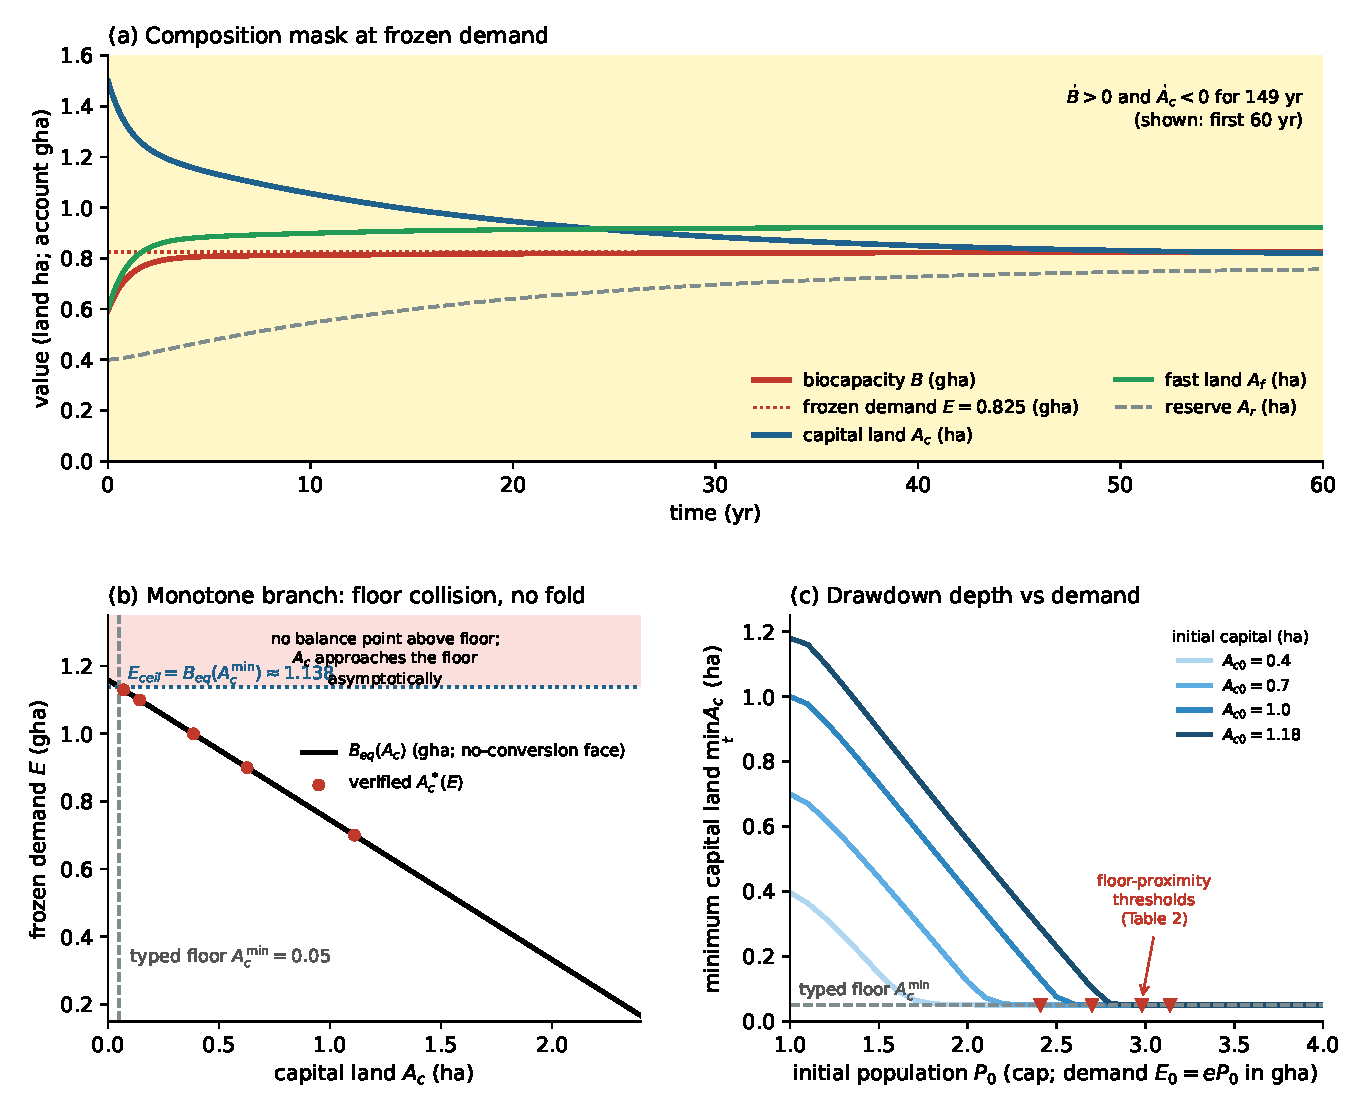
\includegraphics[width=\textwidth]{fig1_model_dynamics}
\caption{Baseline model results (Table~\ref{tab:params}). Account amounts $B$ and $E$ are in gha, land areas are in ha, and population is in cap. (a) Frozen demand ($E=0.825$\,gha), restoration off, and initial conditions $A_{f0}=0.6$\,ha, $A_{c0}=1.5$\,ha, and $q_0=0.9$. $B$ rises from $0.594$ to $0.825$\,gha as $A_c$ falls from $1.500$ to $0.808$\,ha and $A_f$ rises from $0.600$ to $0.923$\,ha. Shading marks the interval with $\dot B>0$ and $\dot A_c<0$ (about $149$\,yr; only the first $60$\,yr are shown). Within $25$\,yr, $98\%$ of the rise in $B$ and $85\%$ of the fall in $A_c$ occur. (b) Fixed-demand balance relation $B_{eq}(A_c)$; the listed balance areas are $A_c^*(E)=1.110$, $0.626$, $0.385$, $0.143$, and $0.070$\,ha at $E=0.70$, $0.90$, $1.00$, $1.10$, and $1.13$\,gha. The curve meets the minimum $A_c=0.05$\,ha at $\Eceil\approx1.138$\,gha; no balance point is admissible at higher demand. (c) Endogenous-demand runs with $\tau_g=20$\,yr, $\tau_p=25$\,yr, and $\chi_r=0.10$\,gha$^{-1}$\,yr$^{-1}$. In the tested runs, the sampled minimum area varies monotonically with $P_0$ for each initial area $A_{c0}$ ($E_0=eP_0$); the finite grid does not establish a general continuity theorem. The floor is approached asymptotically. Triangles mark the proximity values in Table~\ref{tab:model}, defined as within $10^{-6}$\,ha of the floor; no discontinuity is observed.}
\label{fig:model}
\end{figure}

\subsection{Fixed demand leads to a minimum-area boundary, not a fold}\label{sec:ceiling}

Once population reaches carrying capacity, $P=K=B/e$ and demand $E=eP$ equals biocapacity $B$; the shortfall then closes. Conversion is therefore transient in the endogenous-population runs. To isolate how the balance point changes with demand, we also fix $E$ and analyze a reduced land system. The constraint $A_c\ge\Acmin$ is a \emph{typed floor}: it protects one land class, not the aggregate.

\begin{proposition}[Balance point, demand ceiling and affine deficit-side dynamics]\label{prop:ceiling}
For this reduced comparison, hold demand at $E$, switch off the technology boost and restoration, set debt $D=0$, and fix quality at $q=q_{\max}$. Under the projected law, $q_{\max}$ is the limit for an admissible history with $q(0)>0$; the all-zero history remains at zero (SI~\S S2.3). Let $k=\mu/(\mu+\eta_f)$ and
\begin{equation}\label{eq:Beq}
B_{eq}(A_c)=b_{f0}\,k\,(A_{tot}-A_c)+b_cA_c=b_{f0}kA_{tot}-(b_{f0}k-b_c)A_c .
\end{equation}
\begin{enumerate}[label=(\roman*)]
\item At a land-flow equilibrium with no conversion ($S=0$) and $R_{rc}=0$, reserve-to-fast maintenance balances fast-land retirement. Since $S=0$ means $B\ge E$, it includes both the equality balance point and any feasible surplus allocation. The maintenance balance gives $A_f=k(A_{tot}-A_c)$ and $A_r=(1-k)(A_{tot}-A_c)$, where $k=\mu/(\mu+\eta_f)$, and the resulting total is $B_{eq}(A_c)$. If $b_{f0}k>b_c$, this total decreases as $A_c$ increases, so the equality equation $B_{eq}(A_c^*)=E$ has at most one solution:
\begin{equation}\label{eq:Acstar}
A_c^*(E)=\frac{b_{f0}kA_{tot}-E}{b_{f0}k-b_c}.
\end{equation}
The algebraic solution is feasible when $B_{eq}(A_{tot})\le E\le\Eceil$, where $\Eceil=B_{eq}(\Acmin)$. It lies above the minimum area exactly when $E<\Eceil$. At lower demand, the algebraic root lies above $A_{tot}$, and every feasible no-conversion allocation already supplies at least $E$.
\item While shortfall is positive and conversion is not yet limited by the minimum-area constraint, the land subsystem is affine in $z=(A_f,A_c)$: $\dot z=Jz+c$, with
\begin{equation}\label{eq:J}
J=\begin{pmatrix}-\tconv^{-1}-\mu-\eta_f & -\mu-\dfrac{b_c}{b_f\tconv}\\[8pt] \tconv^{-1} & \dfrac{b_c}{b_f\tconv}\end{pmatrix},
\qquad \det J=\frac{\mu+\eta_f}{\tconv}\Big(k-\frac{b_c}{b_f}\Big),
\end{equation}
and $\operatorname{tr}J<0$. The matrix does not depend on demand or on the current state. Its determinant is positive exactly when $B_{eq}$ decreases, and its fixed point is the balance point in (i). For $B_{eq}(A_{tot})\le E<\Eceil$, trajectories that remain in this regime approach that point at rates set by the eigenvalues of $J$. For $E>\Eceil$, the balance point would lie below the allowed minimum: $A_c$ approaches $\Acmin$ asymptotically and the shortfall tends to $S^*=E-\Eceil>0$. Thus the reduced balance curve meets the minimum-area boundary; it does not turn back or form a fold. The leading eigenvalue does not approach zero at $E=\Eceil$, and the reduced equilibrium relation has no hysteresis. These conclusions hold under the stated assumptions and do not imply that the realized land allocation is independent of its history.
\item Above the demand ceiling, with degradation active, debt approaches a unique value $D^*(E)$ satisfying $\eta D=E-B_{eq}(\Acmin;D)$, where $B_{eq}(\cdot;D)$ uses yield $b_{f0}e^{-\alpha D}$. This result requires $\eta>\alpha b_{f0}k(A_{tot}-\Acmin)$; the equilibrium debt increases with demand.
\end{enumerate}
\end{proposition}

\begin{proof}
(i) With $S=0$ and $R_{rc}=0$, \eqref{eq:Af} gives $\mu A_r=\eta_fA_f$, hence $A_r/A_f=\eta_f/\mu$ and, with $A_r=A_{tot}-A_f-A_c$, $A_f=k(A_{tot}-A_c)$; substituting into \eqref{eq:B} with $q=q_{\max}$ ($\Ups=b_c$) and $D=0$ gives $B=B_{eq}(A_c)$, and $S=0$ requires $B\ge E$. Strict monotonicity and \eqref{eq:Acstar} follow from $b_{f0}k>b_c$. (ii) On the deficit side $u_c=(E-b_fA_f-b_cA_c)/(b_f\tconv)$ is affine in $z$; substituting into \eqref{eq:Ac}--\eqref{eq:Af} with $A_r=A_{tot}-A_f-A_c$ gives $J$ and a constant vector $c$ by direct differentiation; $\det J$ follows by expansion, and $\operatorname{tr}J=-\tconv^{-1}(1-b_c/b_f)-\mu-\eta_f<0$ for $b_c<b_f$. The fixed point solves $u_c=0$ and $\mu A_r=\eta_fA_f$, i.e.\ it is the balance point. Because $J$ is constant, convergence rates are constant along the branch. (iii) The map $D\mapsto\eta D+B_{eq}(\Acmin;D)-E$ is continuous, negative at $D=0$ when $E>\Eceil$, tends to $+\infty$, and is strictly increasing when $\eta>\alpha b_{f0}k(A_{tot}-\Acmin)\ge-\partial_DB_{eq}$; hence it has a unique root, which increases with $E$.
\end{proof}

The equality point $B_{eq}(A_c^*)=E$ is unique when feasible, but at fixed exogenous demand every feasible maintenance-balanced allocation with $B_{eq}(A_c)\ge E$ has $S=0$ and no conversion; strict-surplus allocations are a separate no-conversion family, subject to the land bounds. The deficit-side matrix $J$ describes only active-shortfall dynamics, and the switch at $S=0$ means its eigenvalues do not establish two-sided stability of an isolated equality point. In the full endogenous-population model, when $K_{\min}$ is inactive, a positive stationary population also requires $E=B$, so its no-conversion equilibrium family lies on the equality relation with $P$ adjusted to $B/e$. In the baseline run, $R_{rc}=0$ and conversion has no reverse flow: after the shortfall closes, $A_c$ stops falling and remains below its pre-overshoot level. Meanwhile, $q$ evolves separately, so $\Ups(q)$ can still change. This is not perpetual decline at equilibrium and is not a claim about real ecosystems.

At baseline, $k=0.5455$, the balance-branch slope parameter is $b_{f0}k-b_c=0.414$\,gha\,ha$^{-1}$, and the demand ceiling is $\Eceil=1.138$\,gha. Equation~\eqref{eq:Acstar} predicts balance areas of $1.110$, $0.626$, $0.385$, $0.143$, and $0.070$\,ha at demands of $0.70$, $0.90$, $1.00$, $1.10$, and $1.13$\,gha; these match the integrated equilibria (Fig.~\ref{fig:model}b). The eigenvalues of $J$ are real and negative ($\lambda_1=-0.0537$, $\lambda_2=-0.998$\,yr$^{-1}$). Across the tested fast-land yields, $\lambda_1$ shifts only from $-0.0522$ at $b_f=0.60$ to $-0.0556$\,yr$^{-1}$ at $b_f=2.00$ and never changes sign (Table~\ref{tab:model}a).

Above the ceiling, using the same unrounded inputs in both calculations, $E_{\mathrm{ceil}}=1.138409091$\,gha, and $E=E_{\mathrm{ceil}}+0.02=1.158409091$ and $E_{\mathrm{ceil}}+0.10=1.238409091$\,gha give $D^*=1.209655$ and $5.394538$\,gha\,yr. Integration from the maintenance-balanced allocation at $A_c=\Acmin$, with $D(0)=0$, $q=q_{\max}$, $\Delta t=0.1$\,yr and $T=1200$\,yr gives the same values to the displayed precision (SI~\S S2.4). The uniqueness condition holds with margin: $\alpha b_{f0}k(A_{tot}-\Acmin)=0.034$\,yr$^{-1}$, below $\eta=0.05$\,yr$^{-1}$. Under fixed demand, debt therefore saturates rather than growing without bound.

\emph{Critical slowing down} refers to a fold approach in which the slowest return rate tends to zero and the return time $T_{ret}\approx-1/\lambda_1$ grows. That does not occur along this reduced balance branch: its linearization is constant, $\lambda_1$ stays away from zero, and the return time remains near $19$\,yr as $E$ approaches $\Eceil$. The modeled signal is instead $A_c$ approaching its minimum—information an aggregate-only observation cannot provide.

In the tested runs, the sampled minimum $A_c$ varies monotonically with initial population $P_0$ for each starting area $A_{c0}$ (Fig.~\ref{fig:model}c); the finite grid and selected bisections do not establish a general continuity result. The trajectory approaches, but does not cross, the floor because $u_c\le(A_c-\Acmin)/\tconv$. A larger initial capital-land area supports a larger $P_0$ before the run approaches that floor.

Table~\ref{tab:model}b gives the initial populations for which $A_c$ comes within $10^{-2}$, $10^{-4}$, or $10^{-6}$\,ha of its minimum. These tolerance-based values are proximity markers, not abrupt thresholds. At the tightest tolerance, $P_0\approx2.41$, $2.70$, $2.98$, and $3.14$\,cap for $A_{c0}=0.40$, $0.70$, $1.00$, and $1.18$\,ha, respectively. They rise with starting area; no jump appears at any tested tolerance.

At $A_{c0}=1.0$\,ha, the delayed-quality $10^{-6}$\,ha proximity values shift by at most $0.001$\,cap across the tested $\tau_g=5,20,40$\,yr cases (SI Table S2). Under the baseline constant history $q(s)=0.9$ with $\rho_c=0.08$\,yr$^{-1}$, the projected quality paths for $\tau_g=20$ and $40$\,yr are exactly identical: both reach the imposed ceiling at $125/9\approx13.8889$\,yr, before either delay elapses. Their matching outcomes are therefore a saturation-induced degeneracy, not evidence of general delay robustness; the $5$\,yr case is distinct. The restoration comparison is unchanged to three decimals because surplus-gated restoration is inactive while $B<E$ (SI~\S S4).

\begin{table}[!htbp]
\centering\small
\caption{Model results at the baseline parameter set. (a) At $q^*=q_{\max}/2$ ($\Ups(q^*)=0.066$\,gha\,ha$^{-1}$), the table reports $\dconv(q^*)$, the eigenvalues of the deficit-side matrix $J$ in \eqref{eq:J}, and the demand ceiling across a sweep of $b_f$; all other parameters are at baseline. (b) For endogenous-demand runs with $A_{f0}=0.6$\,ha, $q_0=0.9$, $\tau_g=20$\,yr, and $\tau_p=25$\,yr, the table reports the initial population $P_0$ at which the minimum $A_c$ comes within the stated distance of the floor $\Acmin=0.05$\,ha. The first two columns use a $P_0$ grid with step $0.1$ ($\Delta t=0.1$\,yr, $T=400$\,yr); the final column uses bisection with the $10^{-6}$\,ha proximity criterion ($\Delta t=0.05$\,yr, $T=1000$\,yr). In the tested runs, sampled drawdown depth is monotone across the $P_0$ grid (Fig.~\ref{fig:model}c); neither the finite grid nor selected bisections establish general continuity. These values define proximity bands, not a single threshold.}
\label{tab:model}
\begin{tabular}{l l l l l}
\toprule
\multicolumn{5}{l}{(a) Fast-land yield sweep (all rows composition-premium, $\dconv>0$)}\\
$b_f$ (gha\,ha$^{-1}$) & $\dconv(q^*)$ (gha\,ha$^{-1}$) & $\lambda_1$ (yr$^{-1}$) & $\lambda_2$ (yr$^{-1}$) & $\Eceil$ (gha) \\
\midrule
$0.60$ & $+0.534$ & $-0.0522$ & $-0.975$ & $0.804$ \\
$0.85$ (baseline) & $+0.784$ & $-0.0537$ & $-0.998$ & $1.138$ \\
$1.20$ & $+1.134$ & $-0.0547$ & $-1.014$ & $1.606$ \\
$2.00$ & $+1.934$ & $-0.0556$ & $-1.029$ & $2.675$ \\
\bottomrule
\end{tabular}

\medskip
\begin{tabular}{l l l l}
\toprule
\multicolumn{4}{l}{(b) Initial population $P_0$ (cap) at which $\min_tA_c$ approaches $\Acmin$ to within:}\\ 
$A_{c0}$ (ha) & within $10^{-2}$\,ha & within $10^{-4}$\,ha & within $10^{-6}$\,ha \\
\midrule
$0.40$ & $\approx1.8$ & $\approx2.1$ & $\approx2.41$ \\
$0.70$ & $\approx2.2$ & $\approx2.4$ & $\approx2.70$ \\
$1.00$ & $\approx2.6$ & $\approx2.8$ & $\approx2.98$ \\
$1.18$ & $\approx2.8$ & $\approx3.0$ & $\approx3.14$ \\
\bottomrule
\end{tabular}
\end{table}

\subsection{Technology gains are finite; debt depends on the shortfall}\label{sec:bounded}

The technology boost and debt both change fast-land yield $b_f$, but in different ways. The boost has a fixed ceiling. Debt can accumulate while a shortfall persists, then approaches a finite level if that shortfall settles.

\begin{proposition}[The technology boost is capped; debt depends on the shortfall]\label{prop:bounded}
Under \eqref{eq:bf}--\eqref{eq:Tb}:
\begin{enumerate}[label=(\roman*)]
\item The technology factor $(b_{f0}+T_b(t))/b_{f0}$ stays between $1$ and $1+\Delta b/b_{f0}$. Its log-scale gain is therefore bounded by $\ln(1+\Delta b/b_{f0})$ for all time ($0.78$ at baseline).
\item Debt satisfies $D(t)\le\max\{D(0),\ \sup_{s\le t}\pos{E-B}(s)/\eta\}$. If the shortfall settles at $S^*$, then $D$ tends to $S^*/\eta$. The resulting reduction in fast-land yield depends on the size of that sustained shortfall.
\item The debt-related yield loss exceeds the largest possible technology gain once the sustained shortfall exceeds $S^\dagger=(\eta/\alpha)\ln(1+\Delta b/b_{f0})$, which is $1.30$\,gha at baseline.
\end{enumerate}
For the additive comparator $b_f=b_{f0}+T_b-\alpha_{\mathrm{add}}D$, where $\alpha_{\mathrm{add}}$ is a distinct coefficient with units ha$^{-1}$\,yr$^{-1}$, the two effects enter symmetrically; the comparison in (iii) then reduces to $\Delta b$ versus $\alpha_{\mathrm{add}}D^*$. The asymmetry above follows from the model's multiplicative form.
\end{proposition}

\begin{proof}
(i) is $0\le T_b\le\Delta b$. (ii) From \eqref{eq:D}, $\dot D\le\bar S-\eta D$ with $\bar S=\sup_{s\le t}\pos{E-B}$, so $D(t)\le\max\{D(0),\bar S/\eta\}$ by comparison; if $\pos{E-B}\to S^*$ then $D\to S^*/\eta$. (iii) compares $\alpha S^*/\eta$ with $\ln(1+\Delta b/b_{f0})$.
\end{proof}

With fixed demand and a persistent shortfall, $D$ approaches $S^*/\eta$; larger shortfalls imply higher debt. At baseline, the asymptotic sustained-shortfall crossover is $S^\dagger\approx1.3$\,gha. It is a scenario-specific comparison, not a transient trajectory threshold: the relative effect along a run depends on $D(0)$, demand history, and the summary window. Debt nevertheless reduces fast-land yield over time.

A technology boost can raise $B$ and carrying capacity; delayed population growth may raise demand too. Peak debt therefore depends on initial population and the summary window. In the matched SI~\S S8 experiment, for $P_0=1.0$\,cap, peak debt over $0$--$250$\,yr is $0.02020$\,gha\,yr with the boost and $0.00813$\,gha\,yr without it (ratio $2.49$). For $P_0=1.2$\,cap, the full-run maximum is lower with the boost ($0.05104$ versus $0.06122$\,gha\,yr), but the maximum after the $40$\,yr wave midpoint is higher ($0.02518$ versus $0.01085$\,gha\,yr; ratio $2.32$). These are conditional model results, not forecasts or empirical estimates.

\subsection{Recovery requires an explicit, gated restoration flow}\label{sec:recovery}

Conversion moves land from capital to fast use. The model has no route back to capital land unless restoration $R_{rc}$ is active; fast-land retirement returns land to reserve instead. Lowering population, footprint, or shortfall therefore does not, by itself, reverse earlier conversion. With $\chi_r=0$, $A_c$ stays at its post-conversion level.

In the projected delayed-quality run ($A_{c0}=1.0$\,ha, $P_0=2.0$\,cap, $\chi_r=0.10$\,gha$^{-1}$\,yr$^{-1}$, $T=400$\,yr), $A_c$ falls to about $0.398$\,ha and then recovers to $A_c(T)=0.677$\,ha. The recovery fraction is $\mathcal R_c=(A_c(T)-A_c^{\mathrm{deg}})/(A_c^{\mathrm{init}}-A_c^{\mathrm{deg}})=0.46$, matching the delayed-quality recovery table in the Supplementary Information (Table S5; $\Delta t=0.1$\,yr).

The two restoration gates operate under different conditions. Surplus-gated restoration is inactive during a shortfall, but may continue after a surplus opens while population adjusts. Reaching a specified endpoint therefore requires a target-limited rule (SI~\S S4.4). Deficit-gated restoration acts during shortfall, when supply is already insufficient. At the tested rates, conversion outpaces restoration and drawdown continues. The result depends on timing and rates; neither gate is universally preferable.

\subsection{NFA account composition, 1961--2023}\label{sec:empirical}

For the primary empirical analysis, we use complete world observations in NFA Edition 2026, results and metadata version 1.0, and exclude the estimated 2024--2025 values. Our 1961--2022 sensitivity uses the same account edition and population series.

Between 1961 and 2023, total biocapacity account value $B$ rises from $9.7254\times10^9$ to $12.1428\times10^9$\,gha ($24.86\%$; $\Delta\ln B=+0.221997$). Population grows from $3.06487$ to $8.09173$ billion. Over the same interval, $B/P$ falls from $3.17319$ to $1.50065$\,gha\,person$^{-1}$ ($52.71\%$; $\Delta\ln(B/P)=-0.748840$). The Global Ecological Footprint of Production per person ($E_{\mathrm{prod}}/P$) rises from $2.19700$ to $2.56462$\,gha\,person$^{-1}$ ($16.73\%$). Meanwhile, $E_{\mathrm{prod}}/B$ rises from $0.69236$ to $1.70901$, first exceeding one in 1973.

The exact identity $\Delta\ln B=\Delta\ln P+\Delta\ln(B/P)$ yields $+0.970837-0.748840=+0.221997$. It separates population-scale change from change in biocapacity per person, but does not explain their causes. The same-edition 1961--2022 sensitivity gives $\Delta\ln B=+0.219497$, a $52.41\%$ fall in $B/P$, a $17.70\%$ rise in $E_{\mathrm{prod}}/P$, and 1973 as the first year with $E_{\mathrm{prod}}/B>1$ (SI~\S S5).

\begin{figure}[!htbp]
\centering
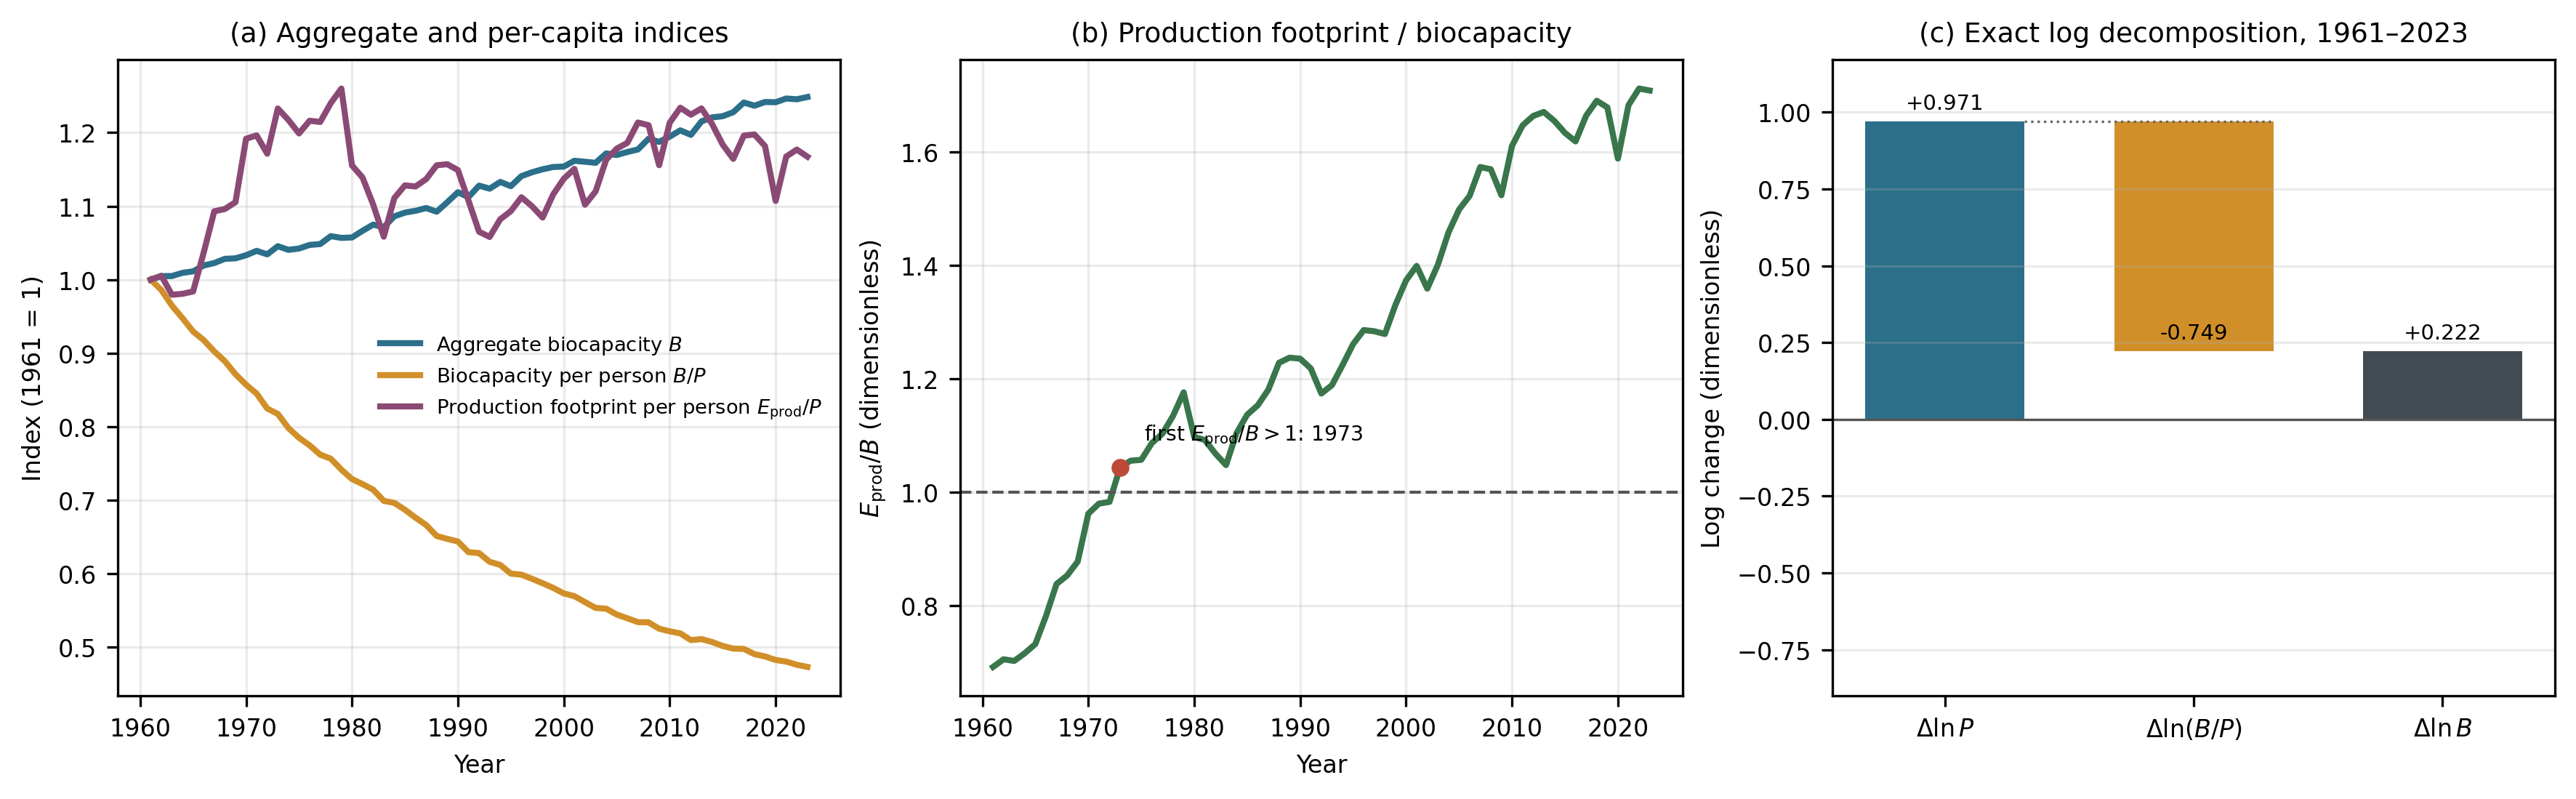
\includegraphics[width=\textwidth]{fig2_nfa_aggregation_face}
\caption{Aggregate and per-capita movements in NFA Edition 2026 (world, 1961--2023; complete observations). $B$ is total biocapacity, $E_{\mathrm{prod}}$ is the workbook's Global Ecological Footprint of Production, and $P$ is the single UN PopStat population series; per-capita values are calculated from totals. (a) Indices (1961 $=1$) of $B$, $B/P$, and $E_{\mathrm{prod}}/P$. (b) $E_{\mathrm{prod}}/B$, first above one in 1973. (c) Exact log identity $\Delta\ln B=\Delta\ln P+\Delta\ln(B/P)$. Account values are in gha; plotted indices, ratios, and log changes are dimensionless. The 2024--2025 estimated rows are excluded.}
\label{fig:aggregation}
\end{figure}

The component series show how NFA account composition changed (Fig.~\ref{fig:composition}; Table~\ref{tab:nfa_components}). Cropland contributes $+24.06$ percentage points to the aggregate's $+24.86\%$ change—about $96.8\%$ of the net percentage change. \mbox{Forest biocapacity} contributes $-5.95$ points, grazing land $-0.27$, fishing grounds $-0.42$, and built-up land $+7.44$. The non-cropland account sum, which includes built-up land, is nearly unchanged ($1.0092\times$, or $+0.80$ points) because the built-up increase offsets declines elsewhere. These are changes in account values. They do not establish changes in forest biomass, soil condition, wetland extent, fish biomass, or model area $A_c$. Built-up land is an account class, not ecological capital. Component values sum to total biocapacity within workbook rounding at both endpoints.

\begin{table}[!htbp]
\centering\footnotesize
\caption{NFA Edition 2026 biocapacity-account endpoint ratios and contributions. Contributions are $100\,[B_i(T)-B_i(1961)]/B(1961)$ percentage points; endpoint ratios are $B_i(T)/B_i(1961)$. The 2022 sensitivity is from the same edition. All entries are account values, not physical-stock measurements.}
\label{tab:nfa_components}
\begin{tabularx}{\textwidth}{@{}Xrrrr@{}}
\toprule
Component & \shortstack{2023\\ratio} & \shortstack{2023 contribution\\(pp of $B_{1961}$)} & \shortstack{2022 sensitivity\\ratio} & \shortstack{2022 contribution\\(pp of $B_{1961}$)} \\
\midrule
Cropland & 2.8701 & $+24.0577$ & 2.8514 & $+23.8183$ \\
Grazing land & 0.9828 & $-0.2688$ & 0.9815 & $-0.2890$ \\
Forest biocapacity & 0.8996 & $-5.9525$ & 0.9019 & $-5.8137$ \\
Fishing grounds & 0.9627 & $-0.4212$ & 0.9596 & $-0.4559$ \\
Built-up land$^{\dagger}$ & 8.7935 & $+7.4416$ & 8.6298 & $+7.2854$ \\
Non-cropland sum$^{\dagger}$ & 1.0092 & $+0.7990$ & 1.0083 & $+0.7267$ \\
\midrule
Total biocapacity & 1.2486 & $+24.8568$ & 1.2454 & $+24.5450$ \\
\bottomrule
\end{tabularx}
\begin{flushleft}\footnotesize
$^{\dagger}$Built-up land is not ecological capital; the non-cropland account sum includes it. Component sums match total biocapacity within workbook rounding. \end{flushleft}
\end{table}

\begin{figure}[!htbp]
\centering
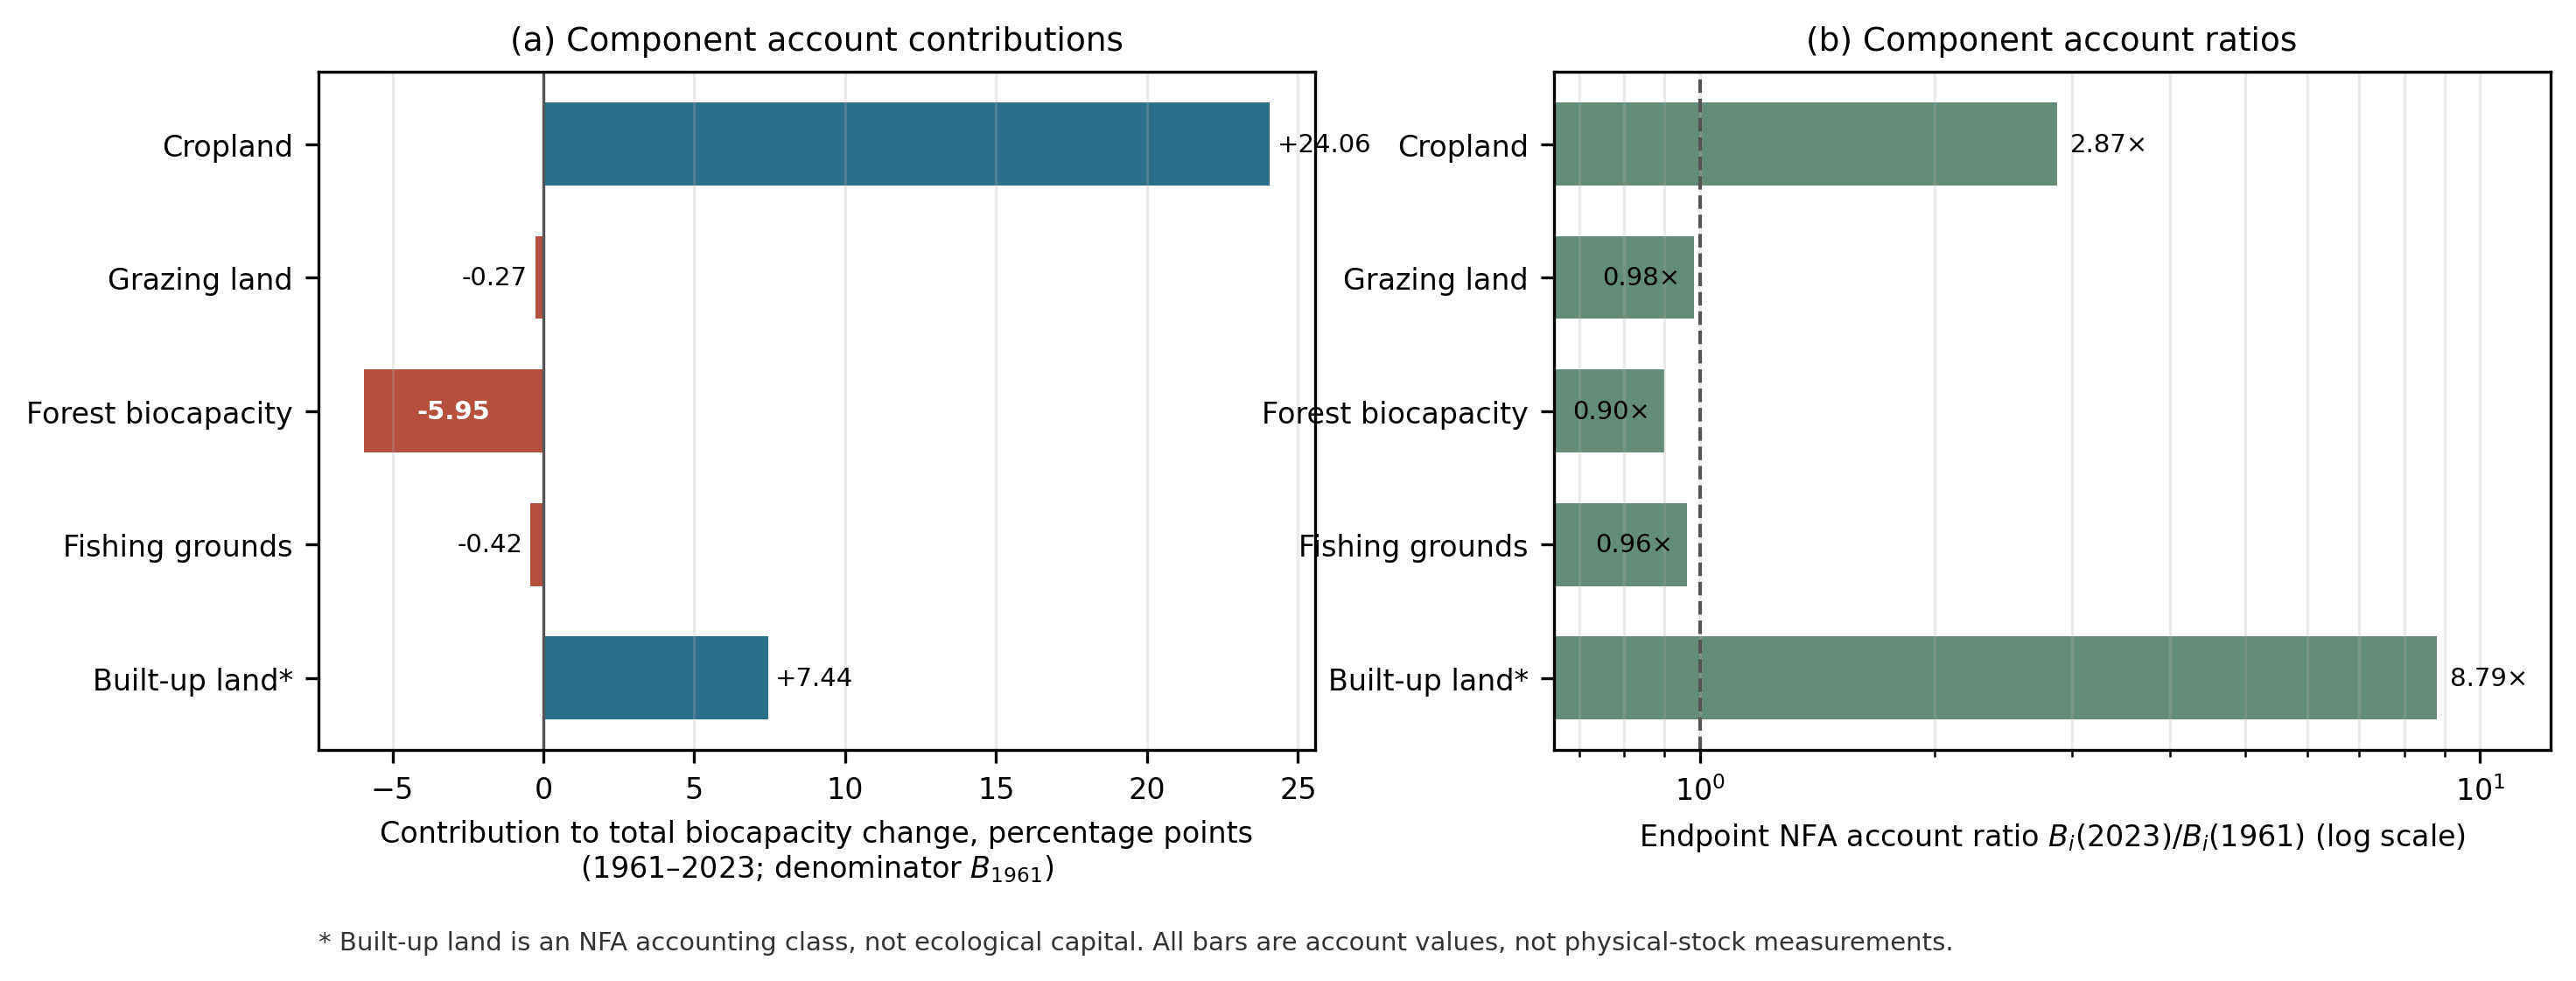
\includegraphics[width=0.95\textwidth]{fig3_composition_attribution}
\caption{NFA Edition 2026 land-type biocapacity-account changes, world, 1961--2023. (a) Component contributions in percentage points of $B_{1961}$. (b) Endpoint ratios $B_i(2023)/B_i(1961)$. “Forest biocapacity” is the workbook's exact label. All bars are account values, not measurements of physical stocks; built-up land is an NFA accounting class, not ecological capital.}
\label{fig:composition}
\end{figure}

We also use external cropland area and cereal yield to build an illustrative proxy for the fast-land contribution (SI~\S S5). Anchoring it to the measured 1961 NFA cropland share ($\phi_0=0.128647$, about $12.86\%$), the exact log-change split assigns $+0.268662$ to the cereal-yield index, $+0.037710$ to cropland area, and $-0.084375$ to the residual. Together these sum to $\Delta\ln B=+0.221997$. The identity is exact for this proxy, but its allocation changes with the anchor and is not a physical-stock attribution.

\subsection{Falsifiable predictions}\label{sec:predictions}

The model yields five testable predictions. Aggregate $B$ alone cannot test them: the composition mechanism requires independent observations or defensible proxies for $A_c$, fast-land area, and yield; testing delay, recovery, and demand-threshold predictions also requires relevant time series and intervention or demographic data.
\begin{enumerate}[label=P\arabic*.,leftmargin=2.2em]
\item \textbf{Conversion can raise the total under a specific condition.} In the baseline frozen-demand run, $\dot A_c<0$ while $\dot B>0$ for a finite interval (Fig.~\ref{fig:model}a). Conversion adds to $B$ exactly when $\dconv>0$, although other flows, quality, debt, technology, and restoration determine the net change. With baseline shares $\sigma_f=\sigma_c=1$, conversion requires demand to exceed total biocapacity ($R_B=E/B>1$). The reserved-share extension can permit conversion when $R_B\le1$, but that is not a baseline result. A composition mask is rising $B$ with falling $A_c$; a liquidation mask is steady $E$ with falling $A_c$. The two patterns may overlap but are not interchangeable. The sign of $\dconv$ describes conversion's contribution, not necessarily the net change in $B$.
\item \textbf{The duration depends on model rates, not a universal horizon.} The slow return rate $\lambda_1$ (along with $\tconv$, $\mu$, $\eta_f$, and $b_c/b_f$) sets the timescale; $\dconv$ and the initial shortfall affect the size of the change. In the baseline, most conversion occurs within one to two e-folding times, when the remaining gap shrinks by a factor of $e$.
\item \textbf{The reduced model has no fold-type early warning.} Return time does not grow as demand approaches the ceiling, and drawdown depth changes continuously with demand (Fig.~\ref{fig:model}c). The model instead signals that $A_c$ is approaching its minimum. It predicts no fold-related warning before that boundary.
\item \textbf{The baseline 20/40-year comparison is saturation-induced.} At $q(s)=0.9$, $\rho_c=0.08$\,yr$^{-1}$ and $q_{\max}=1$, the projected quality reaches its imposed ceiling at $125/9\approx13.8889$\,yr, before either $\tau_g=20$ or $40$\,yr elapses. Those quality paths and matched outcomes therefore coincide; the $\tau_g=5$\,yr case is distinct. The finite comparison does not establish general delay robustness (SI Table S2).
\item \textbf{Recovery requires a return flow.} Lower demand alone does not restore capital-land area. The model needs an explicit restoration flow. A surplus-gated flow is inactive during shortfall, whereas a deficit-gated flow can further reduce provision.
\end{enumerate}
\clearpage
\section{Discussion}\label{sec:discussion}

\subsection{What the two-land model shows}

The two-land model yields three results relevant to human--environment models \citep{Schaefer1954,May1973,Meadows1972,Meadows2004,WackernagelRees1996,BranderTaylor1998}. First, conversion can add to total biocapacity while $A_c$ falls. Whether $B$ rises overall also depends on other land flows and quality change; Proposition~\ref{prop:mask} gives the exact condition for the conversion term. The technology boost is capped, while debt depends on the magnitude and duration of shortfall (Proposition~\ref{prop:bounded}).

Second, under the reduced fixed-demand assumptions ($q=q_{\max}$, $D=0$, technology boost off, and no restoration), the equality balance relation declines steadily with $A_c$ until it meets the area floor. It does not fold back. The absence of a fold or critical slowing applies to this equality relation, not to every trajectory or to the separate surplus no-conversion family. With one-way conversion and no return flow, $A_c$ remains below its pre-overshoot level after conversion stops, although it no longer declines at the equality point (Table~\ref{tab:neg}). Third, recovery requires an explicit return flow; its effect depends on whether the restoration gate opens during a shortfall or a surplus.

SI~\S S7 gives a separate one-stock comparator. Its state $A$ has comparator-specific units; it is not $A_c$. With constant parameters and no debt, its equilibrium relation is $B(A)=(b+b_G\rho)A-(b_G\rho/A_{\max})A^2$, with $P=B(A)/e$. At the illustrated settings, $b_G\rho<b$, so the relation is monotone; an interior maximum would require other parameters. Its neutral equilibrium family and selected delay trajectories belong only to that formulation. They establish neither a fold nor a universal critical delay or collapse mechanism in the two-land model.

These results also clarify when to expect common early-warning indicators. Rising autocorrelation and variance are associated with approaching a fold \citep{Scheffer2001}. This reduced model reaches a minimum-area boundary instead, so those indicators need not rise first. Their absence would not establish safety. The relevant model signal is the path of $A_c$, which the aggregate alone cannot reveal.

\begin{table}[!htbp]
\centering\footnotesize
\caption{Equilibrium, trajectory, and tested delay-sensitivity properties under the stated assumptions.}
\label{tab:neg}
\begin{tabularx}{\textwidth}{>{\raggedright\arraybackslash}p{0.34\textwidth} l >{\raggedright\arraybackslash}X}
\toprule
Property & Finding & Scope \\
\midrule
Fold on the reduced frozen-demand branch & Absent & $B_{eq}(A_c)$ is strictly monotone; the balance point collides with the typed floor at $\Eceil\approx1.138\,\mathrm{gha}$ (Proposition~\ref{prop:ceiling}) \\
Critical slowing as $E\to\Eceil$ & Absent & The slow eigenvalue remains negative and constant along the reduced branch \\
Hysteresis of the reduced equality relation & Absent on this relation & There is at most one feasible equality point; fixed-demand surplus no-conversion allocations form a separate family, and the deficit-side eigenvalues are one-sided \\
Path dependence of realized $A_c$ & Present, conditional & With $R_{rc}=0$, one-way conversion leaves $A_c$ below its pre-overshoot level after shortfall closure, while $\dot A_c=0$ at equilibrium \\
Discontinuous response to endogenous demand & Not observed & The sampled minimum $A_c$ varies monotonically across tested initial populations; proximity thresholds depend on tolerance. The finite runs do not establish a general continuity theorem \\
Regeneration-delay comparison ($\tau_g$, with $\tau_p=25$\,yr) & Degenerate at 20/40\,yr & Baseline quality reaches its imposed ceiling before either delay elapses, so those paths coincide; $\tau_g=5$\,yr is distinct. This is not general delay robustness (SI Table S2) \\
\bottomrule
\end{tabularx}
\end{table}
\clearpage

\subsection{Measurement implications}

Biocapacity in gha is a value-weighted total, not an inventory of land classes. A $20\%$ increase cannot distinguish modest gains across all components from a large gain in one that offsets losses elsewhere. Proposition~\ref{prop:mask}(iii) formalizes the limit: even with fixed per-hectare yields, the total and the conserved-area constraint leave multiple feasible allocations among fast, capital, and reserve land.

A related transition-assessment study defines a linear compensatory operator and compares perfect substitutability with less-substitutable CES alternatives \citep[Sections~2 and 4 of][]{Abaee2026b}. ECOMOD's $B$ is also a linear sum, but the companion analyzes a different, finite-plan setting. There, the compensatory protocol accepts states even when no single available plan meets every component floor (Theorem~2 in \citet{Abaee2026b}). Theorem~4(iii) in \citet{Abaee2026b} identifies an exact interval of diagonal-gap states on its witness-defined region that each positive elasticity falsely certifies as safe; thus no positive-elasticity member is uniformly safe on that region. If feasibility is required throughout a transition, falling below a land-class minimum remains a violation even if the endpoint later recovers.

For the NFA, these findings concern account composition, not physical stocks. In Edition 2026, total world biocapacity account value $B$ rises $24.86\%$ from 1961 to 2023, while $B/P$ falls $52.71\%$. The Global Ecological Footprint of Production per person ($E_{\mathrm{prod}}/P$) rises $16.73\%$, and $E_{\mathrm{prod}}/B$ first exceeds one in 1973. $B$ and $E_{\mathrm{prod}}$ are annual account amounts in gha, with the annual basis implicit; per-person values are in gha per person, and $E_{\mathrm{prod}}/B$ is dimensionless.

Cropland contributes $+24.06$ percentage points to the total change; Forest biocapacity contributes $-5.95$, grazing land $-0.27$, fishing grounds $-0.42$, and built-up land $+7.44$. The non-cropland sum is nearly flat because these account movements offset one another, including the large built-up-land increase. SI~\S S5 reports the same-edition 1961--2022 comparison. None of these values measures forest biomass or condition, soil carbon, wetland extent, fish biomass, or another physical stock. In particular, a decline in Forest biocapacity does not establish a decline in forest biomass. Built-up land is an NFA accounting class, not ecological capital. The ratios, contributions, vintage, and endpoint sensitivity describe account composition only \citep{Lo2026NFA,Borucke2013,Blomqvist2013,GiampietroSaltelli2014,Galli2016,vdBerghGrazi2015}.

The model result is distinct from the NFA trends. In the frozen-demand baseline (Fig.~\ref{fig:model}a), $A_c$ falls from $1.500$ to $0.807659$\,ha ($46.16\%$), while model $B$ rises from $0.594$ to $0.825$\,gha ($39\%$). Quality $q$ rises from $0.9$ to $1.0$, moving farther above $q^*=q_{\max}/2$, where $\Ups(q)$ peaks. Its per-hectare value therefore falls from $0.05576$ to $0.05000$\,gha\,ha$^{-1}$ ($10.33\%$), and the modeled contribution $\Ups(q)A_c$ falls from $0.08364$ to $0.04038$\,gha ($51.72\%$).

With restoration off, one-way conversion leaves $A_c$ below its starting value after the shortfall closes. It then remains at the lower balance level rather than declining indefinitely. This is a conditional model result, not an observation or estimate of global physical-stock change.

We assembled no common-boundary global physical-stock series for these components and therefore report no physical-stock composite or global decline finding. The SI scoreboard is a specification—not an inventory—with candidate stock, extent, condition, and annual-flow measures and the requirements for comparing them; it contains no endpoint values. Until spatial and temporal boundaries, units, uncertainty, overlap, valuation or normalization, and permitted substitution are specified, these unlike measures should remain a nonadditive vector. SEEA Ecosystem Accounting also reports ecosystem extent and condition separately from ecosystem services and monetary presentations \citep{UN2021SEEA_EA}.

The external cropland-area and cereal-yield series provide an illustrative proxy, not direct measurements of the model's land classes. The proxy is anchored to the 1961 NFA cropland share; cereal yield is a productivity sentinel, not an all-crops measure, and the area and account boundaries do not match by construction. External cropland area $A_f$ is in hectares and index-scaled yield $\hat b_f$ in gha\,ha$^{-1}$, so $X=\hat b_fA_f$ and $C=B-X$ are account amounts in gha. The residual can absorb boundary and calibration differences, other account components, and conversion-factor changes. It is neither $\Ups(q)A_c$ nor a physical-stock measure. Physical interpretation would require independent, boundary-consistent measures of area, condition, yield, and regeneration, together with a validated mapping and valuation. Forest area could inform one part of the effective capital class, but cannot represent the entire class or its condition.

\subsection{Policy controls and limits}

We compare three controls. The rate law in Eq.~(5) already preserves the capital-land floor from safe initial states: for $y=A_c-\Acmin\ge0$, $0\le u_c\le y/\tconv$ and $R_{rc}\ge0$ imply $\dot y\ge-y/\tconv$, hence $y(t)\ge y(0)e^{-t/\tconv}$. The floor is approached asymptotically; a stop is an operational safeguard, not an additional continuous-time guarantee in this model. A ceiling on fast-land area $A_f$ does not by itself enforce the capital-land constraint. Total $B$ cannot reconstruct $A_c$ or implement arbitrary $A_c$-dependent policies, but this information limitation is not a universal control impossibility: a constant no-conversion policy also preserves the floor. Any claim of impossibility while meeting a provision objective must specify the admissible controller class, state uncertainty, and objective.

The restoration gates also behave differently. Surplus-gated restoration is inactive during a shortfall; deficit-gated restoration acts during the shortfall and can reduce provision further. This comparison echoes the distinction between protective and mobilizing institutional feedback in related work \citep{Abaee2026a}. With a common reserved share, $\sigma_f=\sigma_c=\sigma<1$, conversion is inactive while $E\le\sigma B$. With separate shares, the condition is $E\le\sigma_fY_f+\sigma_cY_c$. This reservation applies to annual human-available flow, not to spatially protected area. Half-Earth, by contrast, is a spatial conservation target \citep{Wilson2016}. The connection is only the abstract idea of reservation: the model neither maps protected areas nor evaluates that proposal. Robustness to disturbances and parameter uncertainty remains untested.

\subsection{Relation to prior work}

The ledger companion distinguishes weak and strong sustainability as operating regimes according to whether material loops close at throughput. In its terms, a positive weighted sum ranks outcomes under weak sustainability, whereas componentwise adequacy is the strong-sustainability predicate \citep[Sections~1.1 and 10.1]{Abaee2026c}. ECOMOD's $B$ is an annual biocapacity-account total. The link is an analogy about compensation, not an identity with the companion's material-flow ledger or a complete sustainability classification. The assessment companion studies aggregate measures and typed transition criteria in a separate finite-plan setting \citep{Abaee2026b}; the governance companion studies institutional feedback \citep{Abaee2026a}. The delays here represent ecological regeneration and demographic response, not institutional review.

\subsection{Limitations}

Several limitations set the scope of the results. Ecological-capital land combines unlike assets, so its single quality state, projected regeneration rule, composition diagnostic, and demand ceiling are effective model quantities—not estimates for forests, soils, or wetlands. The quality index is uncalibrated; $q_{\max}=1$ is an imposed admissibility bound, and $\rho_c$ and $\tau_g$ are scenario parameters rather than estimates from recovery studies. Most other parameters are representative rather than fitted. A cross-section cannot identify $b_c$, $b_{G,c}$, and $\rho_c$ separately. Recovery records from different systems and external measurement frameworks are precedents for future ecosystem-specific measurement and modeling only; they do not validate the present equation or parameter values. The records describe regeneration responses, not the delay $\tau_g$. We hold the per-person footprint constant to isolate feedbacks among land, biocapacity, and demand. A changing footprint would require another model extension.

The composition pattern depends on demand and on the mechanisms included here; under the stated assumptions, it is bounded. The exact shortfall switch makes stability at $S=0$ one-sided. Drawdown thresholds are reported as proximity bands because they depend on tolerance and time step. We fix debt repayment at $\eta=0.05$\,yr$^{-1}$; the zero-repayment limit ($\eta\to0$), which removes the debt equilibrium, is not analyzed. NFA accounts combine area and yield and therefore cannot identify them separately. Finally, the current-quality comparator $G_c(q(t))$ is retained only as a sensitivity check; it is not the selected projected delayed-quality model. In the displayed finite comparison it lengthens the demonstration window by $1.3$\,yr and shifts the initial-population threshold by at most $0.001$\,cap (SI~\S S3).

\section{Conclusions}\label{sec:conclusions}

Aggregate biocapacity cannot reveal how its underlying land classes are changing. In the two-land model, conversion raises total $B$ at the margin when fast-land contribution per hectare exceeds capital land's effective value ($b_f>\Ups(q)$), while $A_c$ falls if restoration is off (Proposition~\ref{prop:mask}). Other model terms determine whether total $B$ rises overall. This is a conditional accounting mechanism, not an empirical census of global physical stocks.

The reduced fixed-demand equality relation reaches the specified minimum-area boundary without a fold or critical slowing. This is a statement about that relation, not the separate fixed-demand surplus no-conversion family or every trajectory of the delayed model. Realized paths remain history-dependent: when shortfalls subside and restoration is off, $A_c$ remains below its pre-overshoot level, but it does not continue to decline at the balance point. In the representative baseline run, total model biocapacity rises $39\%$ while ecological-capital area falls $46.16\%$, its per-hectare quality term $\Ups(q)$ falls $10.33\%$, and its modeled contribution $\Ups(q)A_c$ falls $51.72\%$.

Separately, NFA Edition 2026 world account values rise $24.86\%$ between 1961 and 2023, while biocapacity per person $B/P$ falls $52.71\%$ and the production footprint per person rises $16.73\%$. Cropland contributes $+24.06$ percentage points, Forest biocapacity $-5.95$, and Built-up land $+7.44$ as an accounting class. These normalized annual account values are not observations of physical stocks or model $A_c$.

\begin{samepage}
No common-boundary global physical-stock series was assembled, so we report no composite or global physical-stock decline finding. The SI scoreboard sets out candidate measures and comparison requirements; it is not an empirical inventory. Physical measures with different units and boundaries cannot be combined into one stock total without explicit treatment of uncertainty, overlap, valuation or normalization, and allowed substitution. The auxiliary proxy residual $C=B-\hat b_fA_f$ is neither a physical-capital measure nor the model contribution $\Ups(q)A_c$; a future comparison would require independent observations and a validated mapping.\par
\end{samepage}

The practical lesson is to report component accounts alongside the aggregate. Returning to the orchard metaphor, a ledger of annual harvest alone cannot tell whether the trees, roots, and soil that support future harvests have changed. That physical record requires independent, comparable observations; it cannot be inferred from the account total. A harvest total is not a census of the orchard.

\section*{Acknowledgments}

The author thanks Global Footprint Network for making its data publicly available; Mathis Wackernagel for his thoughtful review; the editors of \emph{Ecological Modelling} for their trust and support; and Arena.ai for its ingenuity and online tools.

\section*{Declarations}

\paragraph{Data availability} All empirical inputs are publicly available from the sources cited in the manuscript. Derived analysis data and model code will be deposited in a public GitHub repository and archived in Zenodo.

\paragraph{Funding} No funding was received.

\paragraph{Competing interests} The author declares no competing interests.

\paragraph{CRediT authorship contribution statement} \textbf{Amin Abaee:} Conceptualization; Methodology; Software; Formal analysis; Writing -- original draft; Writing -- review \& editing.

\paragraph{Declaration of generative AI in scientific writing} DeepSeek AI and Claude (Anthropic) assisted with computational-reproducibility checks under the author's supervision; the author reviewed and edited the content and takes full responsibility for the publication.
\begin{thebibliography}{99}
\bibitem[{Abaee(2026a)}]{Abaee2026a} Abaee, A. (2026a). \emph{Governance delay and the stability of harvested stocks: mobilising and protective feedback rules, and the review interval as a design parameter}. Working paper. \href{https://github.com/MIKEAA2020/general-sustainability/blob/2efaa62083f2007dec3446c15c475af88f0925f3/arena%20agent%201/paper%20rewrites/latex/paper4_delay_dynamics_v41.pdf}{Manuscript}.
\bibitem[{Abaee(2026b)}]{Abaee2026b} Abaee, A. (2026b). \emph{Aggregation is a claim, not a presentation: the geometry of the acceptance gap between compensatory and noncompensatory transition assessment}. Working paper. \href{https://github.com/MIKEAA2020/general-sustainability/blob/2efaa62083f2007dec3446c15c475af88f0925f3/arena%20agent%201/paper%20rewrites/latex/paper06_assessment_separation_v71.pdf}{Manuscript}.
\bibitem[{Abaee(2026c)}]{Abaee2026c} Abaee, A. (2026c). \emph{Typed Flux Ledgers and Depletion Arithmetic: Conservation, Componentwise Diagnostics, and the Semantics of Depletion Horizons}. Working paper. \href{https://github.com/MIKEAA2020/general-sustainability/blob/2efaa62083f2007dec3446c15c475af88f0925f3/paper3/latest-2026-09-19/manuscript/paper3_material_ledgers_v50.pdf}{Manuscript}.
\bibitem[{Anderies(2000)}]{Anderies2000} Anderies, J. M. (2000). On modeling human behavior and institutions in simple ecological economic systems. \emph{Ecological Economics}, 35(3), 393--412.
\bibitem[{Becker et al.(2017)}]{Becker2017} Becker, W., Saisana, M., Paruolo, P. \& Vandecasteele, I. (2017). Weights and importance in composite indicators: Closing the gap. \emph{Ecological Indicators}, 80, 12--22.
\bibitem[{Blomqvist et al.(2013)}]{Blomqvist2013} Blomqvist, L., Brook, B. W., Ellis, E. C., Kareiva, P. M., Nordhaus, T. \& Shellenberger, M. (2013). Does the shoe fit? Real versus imagined ecological footprints. \emph{PLoS Biology}, 11(11), e1001700.
\bibitem[{Borucke et al.(2013)}]{Borucke2013} Borucke, M., Moore, D., Cranston, G., Gracey, K., Iha, K., Larson, J., Lazarus, E., Morales, J. C., Wackernagel, M. \& Galli, A. (2013). Accounting for demand and supply of the biosphere's regenerative capacity: The National Footprint Accounts' underlying methodology and framework. \emph{Ecological Indicators}, 24, 518--533.
\bibitem[{Brander and Taylor(1998)}]{BranderTaylor1998} Brander, J. A. \& Taylor, M. S. (1998). The simple economics of Easter Island: A Ricardo--Malthus model of renewable resource use. \emph{American Economic Review}, 88(1), 119--138.
\bibitem[{Calvin and Bond-Lamberty(2018)}]{CalvinBondLamberty2018} Calvin, K. \& Bond-Lamberty, B. (2018). Integrated human--Earth system modeling --- state of the science and future directions. \emph{Environmental Research Letters}, 13(6), 063006.
\bibitem[{Cohen(1995)}]{Cohen1995} Cohen, J. E. (1995). Population growth and Earth's human carrying capacity. \emph{Science}, 269(5222), 341--346.
\bibitem[{Dasgupta(2021)}]{Dasgupta2021} Dasgupta, P. (2021). \emph{The Economics of Biodiversity: The Dasgupta Review.} London: HM Treasury.
\bibitem[{Donges et al.(2017)}]{Donges2017} Donges, J. F., Winkelmann, R., Cornell, S. E., Lucht, W., Dyke, J. G., Rockstr\"om, J., Heitzig, J. \& Schellnhuber, H. J. (2017). Closing the loop: Reconnecting human dynamics to Earth system science. \emph{The Anthropocene Review}, 4(2), 151--157.
\bibitem[{Erb et al.(2017)}]{Erb2017} Erb, K.-H., Luyssaert, S., Meyfroidt, P., Pongratz, J., Don, A., Kloster, S., Kuemmerle, T., Fetzel, T., Fuchs, R., Hasegawa, T., Haberl, H., et al. (2017). Land management: data availability and process understanding for global change studies. \emph{Global Change Biology}, 23(2), 512--533.
\bibitem[{Fischer et al.(2022)}]{Fischer2022} Fischer, S. M., Joy, M. K., Abrahamse, W., Milfont, T. L. \& Petherick, L. M. (2022). The use and misuse of composite environmental indices. \emph{bioRxiv}, 2022.03.15.484501. \url{https://doi.org/10.1101/2022.03.15.484501}.
\bibitem[{Global Footprint Network(2009)}]{GFNStandards2009} Global Footprint Network (2009). \emph{Ecological Footprint Standards 2009}. Global Footprint Network. \url{https://www.footprintnetwork.org/content/uploads/2019/05/Ecological_Footprint_Standards_2009.pdf}.
\bibitem[{Global Footprint Network(2019)}]{GFNGuidebook2019} Global Footprint Network (2019). \emph{Working Guidebook to the National Footprint Accounts 2019}. Global Footprint Network. \url{https://www.footprintnetwork.org/content/uploads/2019/05/National_Footprint_Accounts_Guidebook_2019.pdf}.
\bibitem[{Galli et al.(2016)}]{Galli2016} Galli, A., Giampietro, M., Goldfinger, S., Lazarus, E., Lin, D., Saltelli, A., Wackernagel, M. \& M\"uller, F. (2016). Questioning the ecological footprint. \emph{Ecological Indicators}, 69, 224--232.
\bibitem[{Giampietro and Saltelli(2014)}]{GiampietroSaltelli2014} Giampietro, M. \& Saltelli, A. (2014). Footprints to nowhere. \emph{Ecological Indicators}, 46, 610--621.
\bibitem[{Haberl et al.(2007)}]{Haberl2007} Haberl, H., Erb, K.-H., Krausmann, F., Gaube, V., Bondeau, A., Plutzar, C., Gingrich, S., Lucht, W. \& Fischer-Kowalski, M. (2007). Quantifying and mapping the human appropriation of net primary production in earth's terrestrial ecosystems. \emph{PNAS}, 104(31), 12942--12947.
\bibitem[{Henderson and Loreau(2018)}]{HendersonLoreau2018} Henderson, K. \& Loreau, M. (2018). How ecological feedbacks between human population and land cover influence sustainability. \emph{PLoS Computational Biology}, 14(8), e1006389.
\bibitem[{Hutchings and Reynolds(2004)}]{HutchingsReynolds2004} Hutchings, J. A. \& Reynolds, J. D. (2004). Marine fish population collapses: consequences for recovery and extinction risk. \emph{BioScience}, 54(4), 297--309.
\bibitem[{Krausmann et al.(2013)}]{Krausmann2013} Krausmann, F., Erb, K.-H., Gingrich, S., Haberl, H., Bondeau, A., Gaube, V., Lauk, C., Plutzar, C. \& Searchinger, T. D. (2013). Global human appropriation of net primary production doubled in the 20th century. \emph{PNAS}, 110(25), 10324--10329.
\bibitem[{Lo et al.(2026)}]{Lo2026NFA} Lo, K., Basnet, N., Miller, E., Srikanthalingam, B., Foley, B., Van Berkum, J. L., Long, A. H., Toneva, P., Ermina, M. \& Klinkenberg, C. (2026). \emph{National Ecological Footprint and Biocapacity Accounts, Edition 2026 (1961--2025): Results and metadata, version 1.0.} Prepared for Footprint Data Foundation by researchers at York University and the University of Iceland. Workbook: \url{https://footprint.info.yorku.ca/files/2026/04/NEFBA_Data_global_national_ecological_footprint_biocapacity.xlsx}; release notes: \url{https://footprint.info.yorku.ca/files/2026/04/NEFBA_ReleaseNotes.pdf}; data page: \url{https://footprint.info.yorku.ca/data/}.
\bibitem[{May(1973)}]{May1973} May, R. M. (1973). \emph{Stability and Complexity in Model Ecosystems.} Princeton: Princeton University Press.
\bibitem[{Meadows et al.(1972)}]{Meadows1972} Meadows, D. H., Meadows, D. L., Randers, J. \& Behrens, W. W. (1972). \emph{The Limits to Growth.} New York: Universe Books.
\bibitem[{Meadows et al.(1974)}]{Meadows1974} Meadows, D. L., Behrens, W. W., Meadows, D. H., Naill, R. F., Randers, J. \& Zahn, E. (1974). \emph{Dynamics of Growth in a Finite World.} Cambridge, MA: Wright-Allen Press.
\bibitem[{Meadows et al.(2004)}]{Meadows2004} Meadows, D. H., Randers, J. \& Meadows, D. L. (2004). \emph{The Limits to Growth: The 30-Year Update.} White River Junction, VT: Chelsea Green.
\bibitem[{Meyer(1994)}]{Meyer1994} Meyer, P. S. (1994). Bi-logistic growth. \emph{Technological Forecasting and Social Change}, 47(1), 89--102.
\bibitem[{Meyer and Ausubel(1999)}]{MeyerAusubel1999} Meyer, P. S. \& Ausubel, J. H. (1999). Carrying capacity: A model with logistically varying limits. \emph{Technological Forecasting and Social Change}, 61(3), 209--214.
\bibitem[{Motesharrei et al.(2016)}]{Motesharrei2016} Motesharrei, S., Rivas, J., Kalnay, E., Asrar, G. R., Busalacchi, A. J., Cahalan, R. F., Cane, M. A., Colwell, R. R., Feng, K., Franklin, R. S., et al. (2016). Modeling sustainability: Population, inequality, consumption, and bidirectional coupling of the Earth and human systems. \emph{National Science Review}, 3(4), 470--494.
\bibitem[{Nardo et al.(2008)}]{Nardo2008} Nardo, M., Saisana, M., Saltelli, A., Tarantola, S., Hoffmann, A. \& Giovannini, E. (2008). \emph{Handbook on Constructing Composite Indicators: Methodology and User Guide.} Paris: OECD Publishing.
\bibitem[{Neubauer et al.(2013)}]{Neubauer2013} Neubauer, P., Jensen, O. P., Hutchings, J. A. \& Baum, J. K. (2013). Resilience and recovery of overexploited marine populations. \emph{Science}, 340(6130), 347--349.
\bibitem[{Our~World~in~Data(2026a)}]{OWIDCereal2026} Our~World~in~Data (2026a). \emph{Cereal yield.} FAOSTAT data accessed through Our World in Data; grapher page last updated 25 February 2026; accessed 24 October 2026. \url{https://ourworldindata.org/grapher/cereal-yield}.
\bibitem[{Our~World~in~Data(2026b)}]{OWIDCropland2026} Our~World~in~Data (2026b). \emph{Cropland area.} FAOSTAT data accessed through Our World in Data; grapher page last updated 25 February 2026; accessed 24 October 2026. \url{https://ourworldindata.org/grapher/cropland-area}.
\bibitem[{Poeplau et al.(2011)}]{Poeplau2011} Poeplau, C., et al. (2011). Temporal dynamics of soil organic carbon after land-use change in the temperate zone--carbon response functions as a model approach. \emph{Global Change Biology}, 17(7), 2415--2427.
\bibitem[{Poorter et al.(2016)}]{Poorter2016} Poorter, L., et al. (2016). Biomass resilience of Neotropical secondary forests. \emph{Nature}, 530(7590), 211--214.
\bibitem[{Schaefer(1954)}]{Schaefer1954} Schaefer, M. B. (1954). Some aspects of the dynamics of populations important to the management of the commercial marine fisheries. \emph{Bulletin of the Inter-American Tropical Tuna Commission}, 1(2), 25--56.
\bibitem[{Scheffer et al.(2001)}]{Scheffer2001} Scheffer, M., Carpenter, S., Foley, J. A., Folke, C. \& Walker, B. (2001). Catastrophic shifts in ecosystems. \emph{Nature}, 413(6856), 591--596.
\bibitem[{Simon(1996)}]{Simon1996} Simon, J. L. (1996). \emph{The Ultimate Resource 2.} Princeton: Princeton University Press.
\bibitem[{United Nations et al.(2021)}]{UN2021SEEA_EA} United Nations et al. (2021). \emph{System of Environmental-Economic Accounting---Ecosystem Accounting (SEEA EA).} White cover publication, pre-edited text subject to official editing. New York: United Nations. \url{https://seea.un.org/ecosystem-accounting}.
\bibitem[{United Nations(2022)}]{UN2022} United Nations (2022). \emph{World Population Prospects 2022: Summary of Results.} New York: Department of Economic and Social Affairs, Population Division.
\bibitem[{van den Bergh and Grazi(2015)}]{vdBerghGrazi2015} van den Bergh, J. C. J. M. \& Grazi, F. (2015). Reply to the first systematic response by the Global Footprint Network to criticism: a real debate finally? \emph{Ecological Indicators}, 58, 458--463.
\bibitem[{van den Bergh and Rietveld(2004)}]{vdBerghRietveld2004} van den Bergh, J. C. J. M. \& Rietveld, P. (2004). Reconsidering the limits to world population: Meta-analysis and meta-prediction. \emph{BioScience}, 54(3), 195--204.
\bibitem[{Wackernagel and Rees(1996)}]{WackernagelRees1996} Wackernagel, M. \& Rees, W. (1996). \emph{Our Ecological Footprint: Reducing Human Impact on the Earth.} New Society Publishers.
\bibitem[{Wilson(2016)}]{Wilson2016} Wilson, E. O. (2016). \emph{Half-Earth: Our Planet's Fight for Life.} New York: Liveright.
\end{thebibliography}

\end{document}
